\chapter{Appendix}
%\includepdf[pages={1-4}]{appendix/Piezo.pdf}
\section{Technical documents}

\begin{figure}[h!]\centering 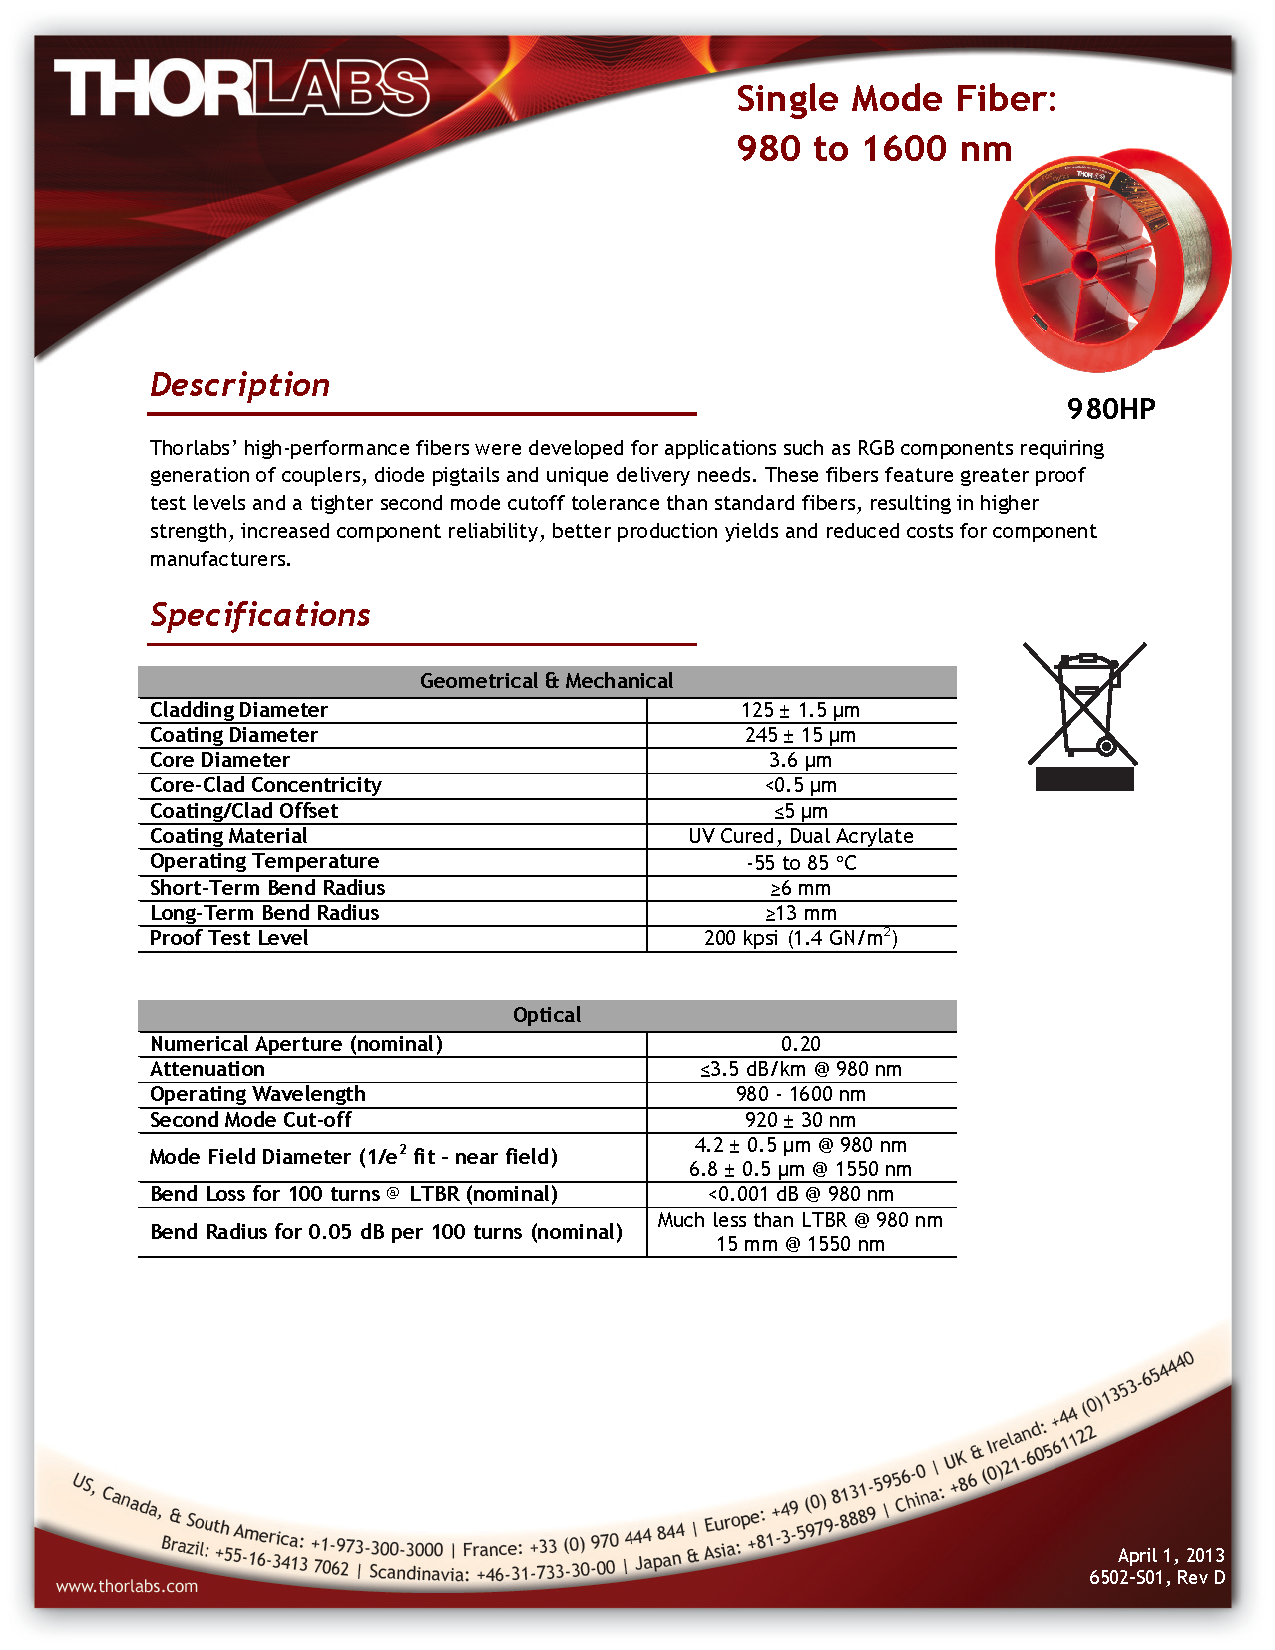
\includegraphics[width=12cm]{appendix/fiber.pdf}
      \caption{Datasheet of the single mode fiber}
\end{figure}

\begin{figure}[h!]\centering 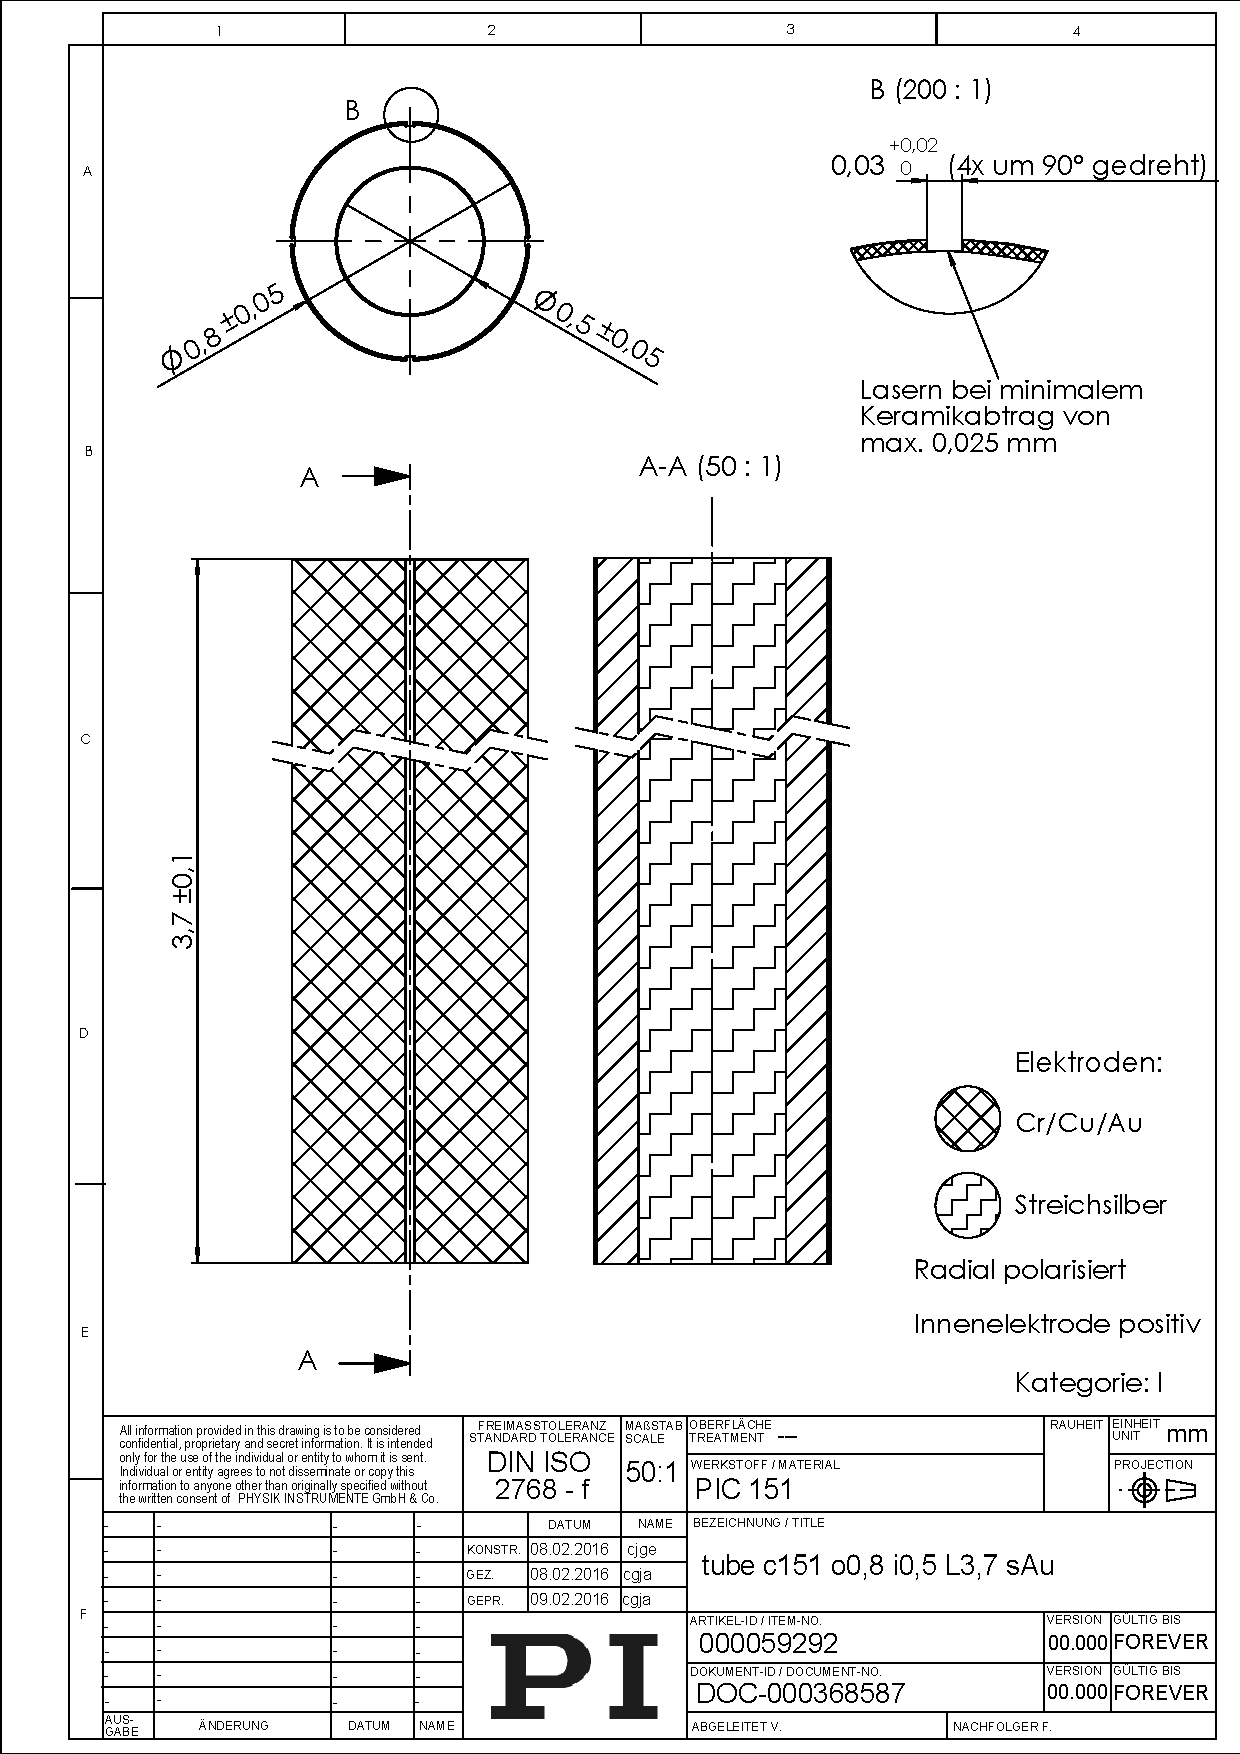
\includegraphics[width=16cm]{appendix/piezo.pdf}
      \caption{Datasheet of the piezoelectric tube}
\end{figure}

\begin{figure}[h!]\centering 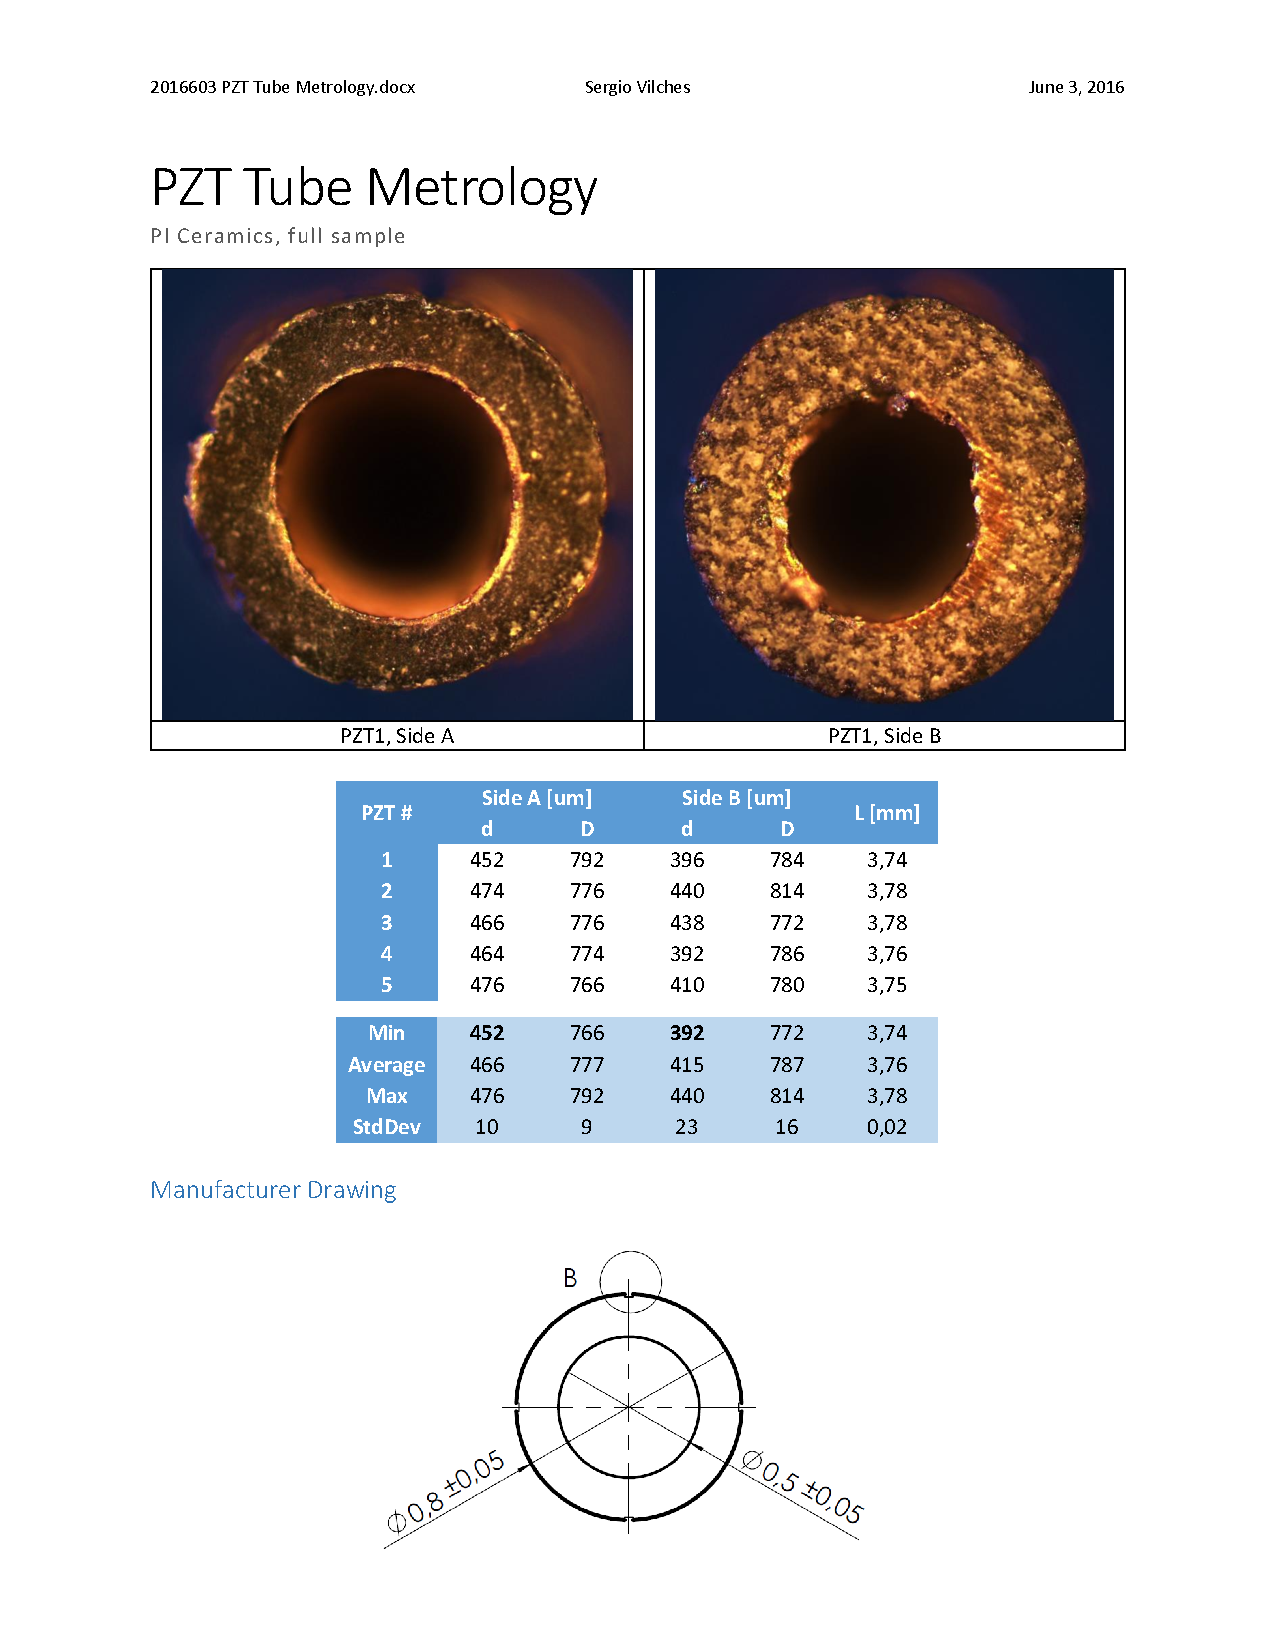
\includegraphics[width=16cm]{appendix/pztPhotos.pdf}
      \caption{Metrology of the acquired piezoeletric tubes}
\end{figure}

\begin{figure}[h!]\centering 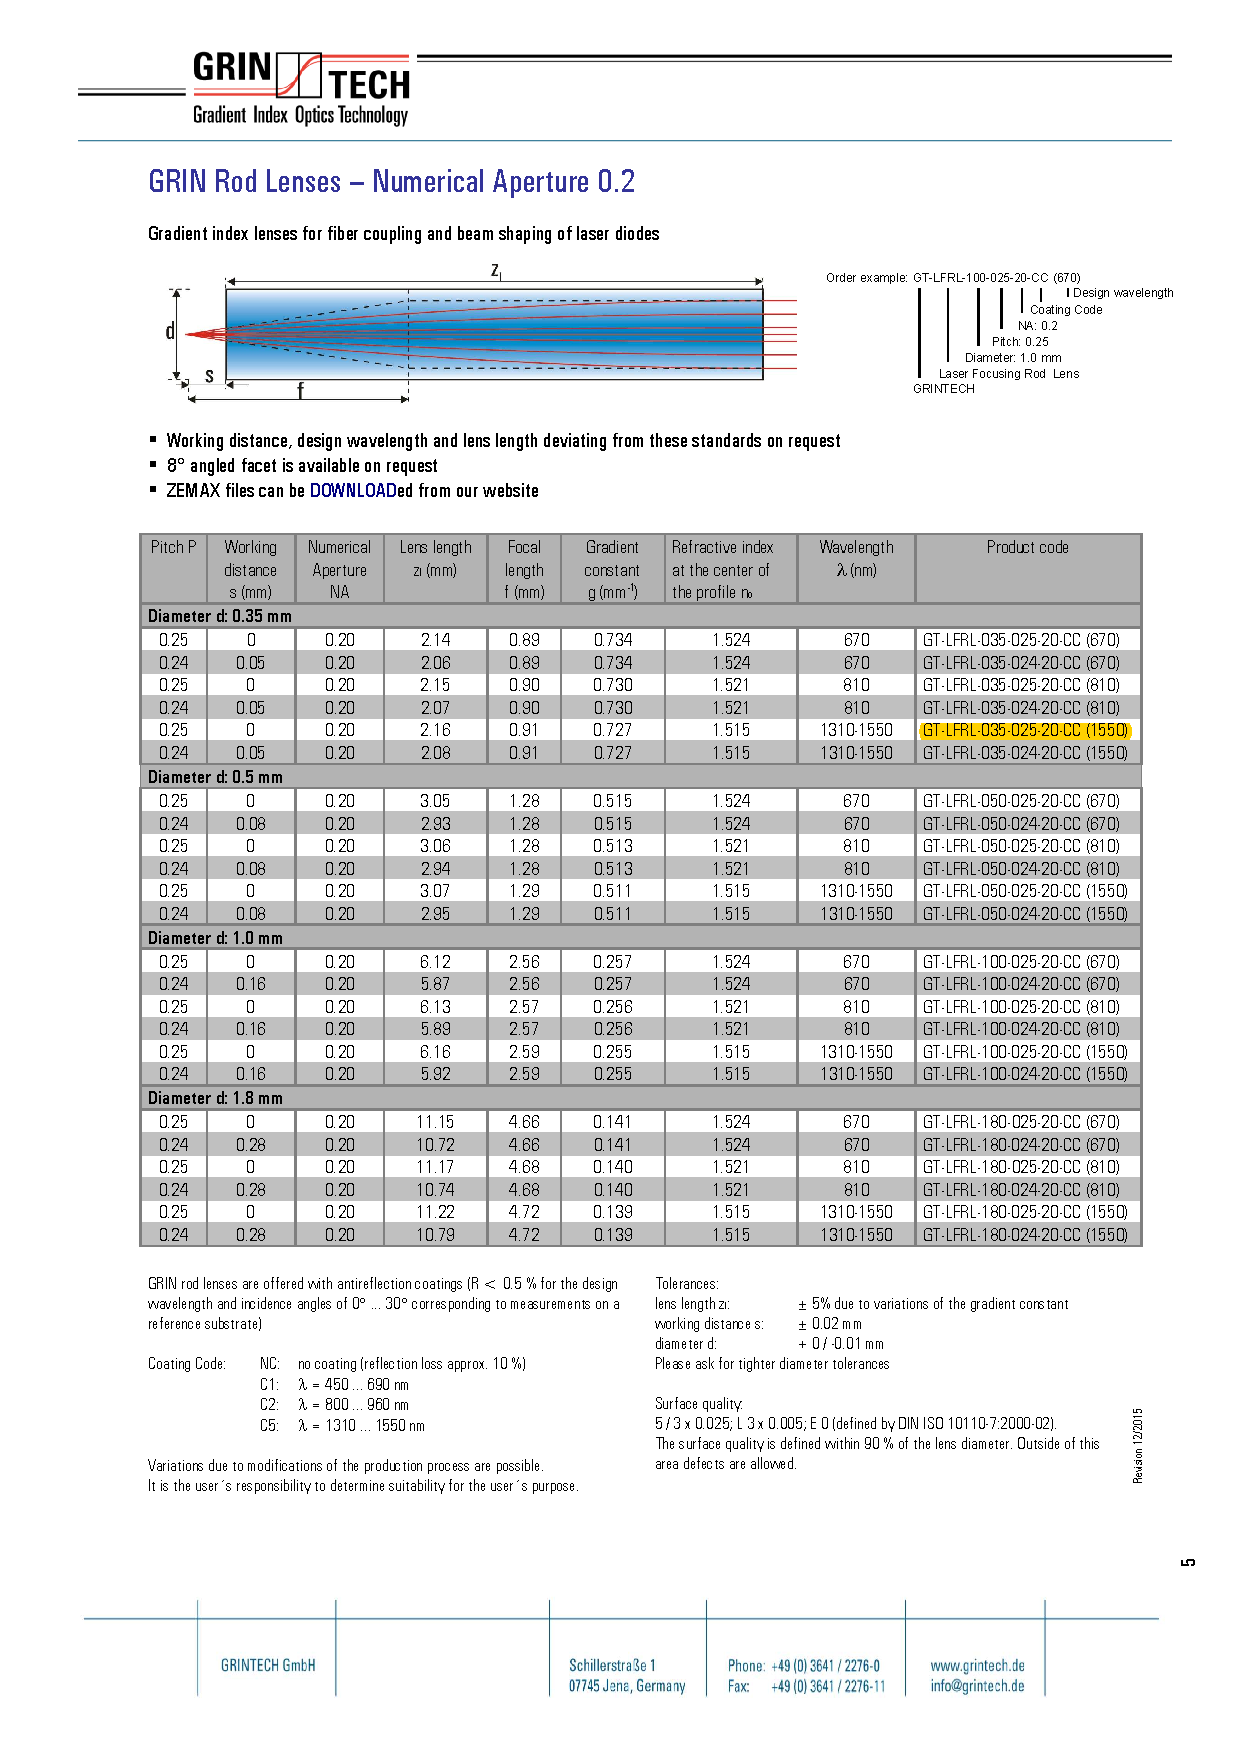
\includegraphics[width=16cm]{appendix/grin.pdf}
      \caption{Datasheet of the 0.2 NA GRIN lenses from GRINTECH \\(GT-LFRL-035-025-20-CC (1550))}
\end{figure}

\begin{figure}[h!]\centering 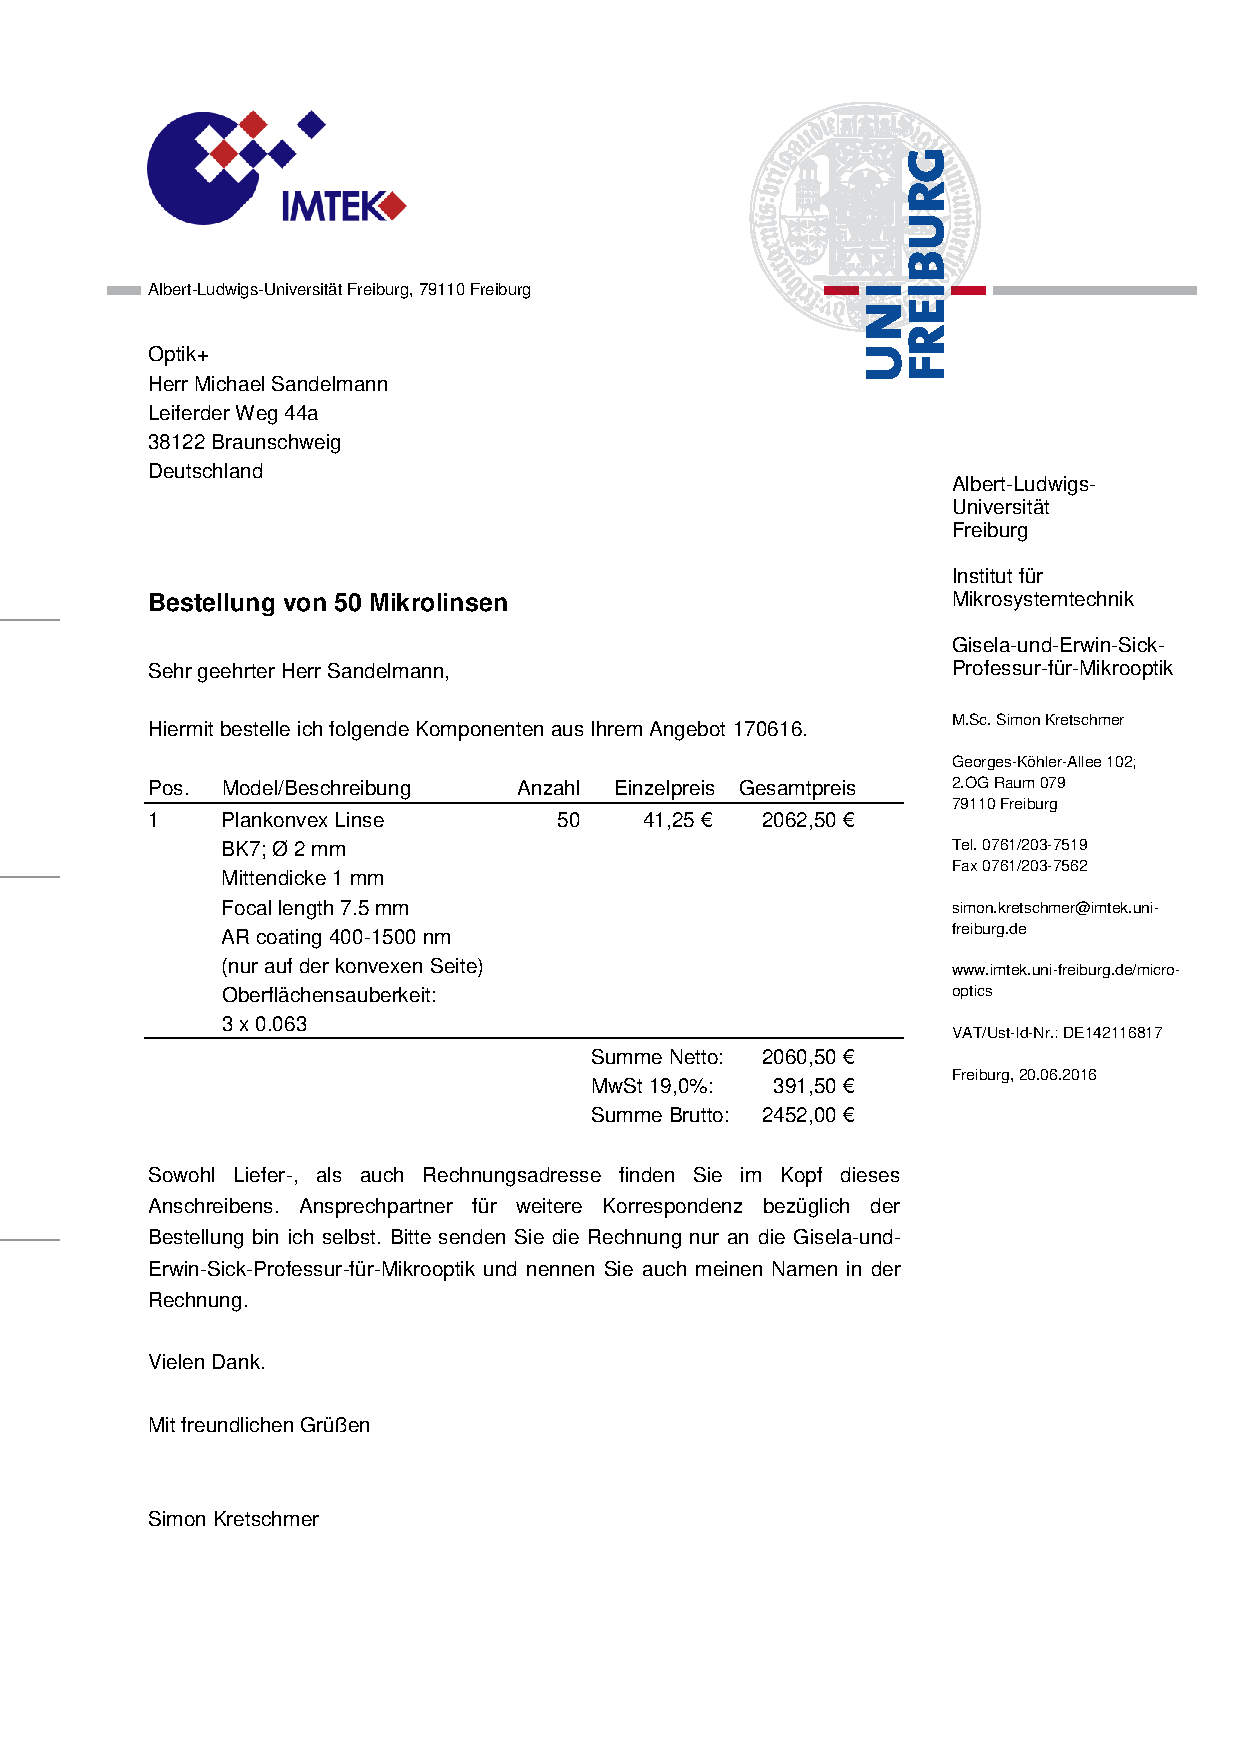
\includegraphics[width=16cm]{appendix/lens.pdf}
      \caption{Order details of the custom designed spherical lenses}
\end{figure}

\clearpage
\section{Cleanroom processes of the polyimide electrodes}
\begin{figure}[h!]\centering 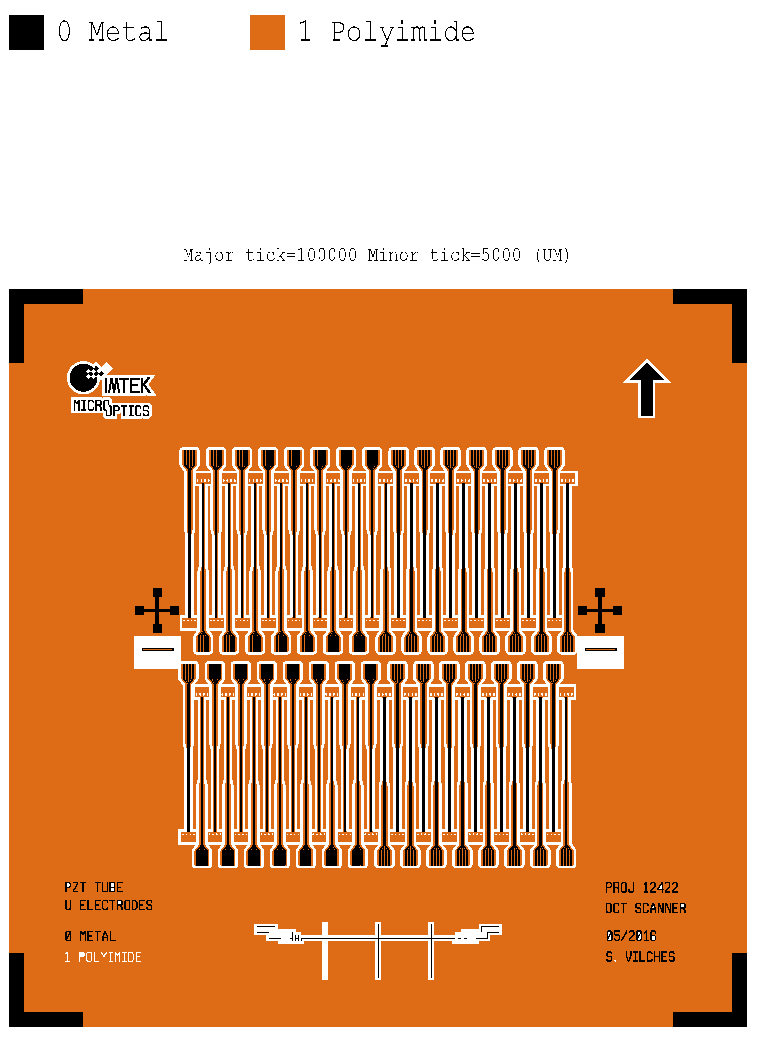
\includegraphics[width=12cm]{appendix/piCuffs.pdf}
      \caption{Maskset used in the manufacturing of the polyimide ribbon cables.}
\end{figure}
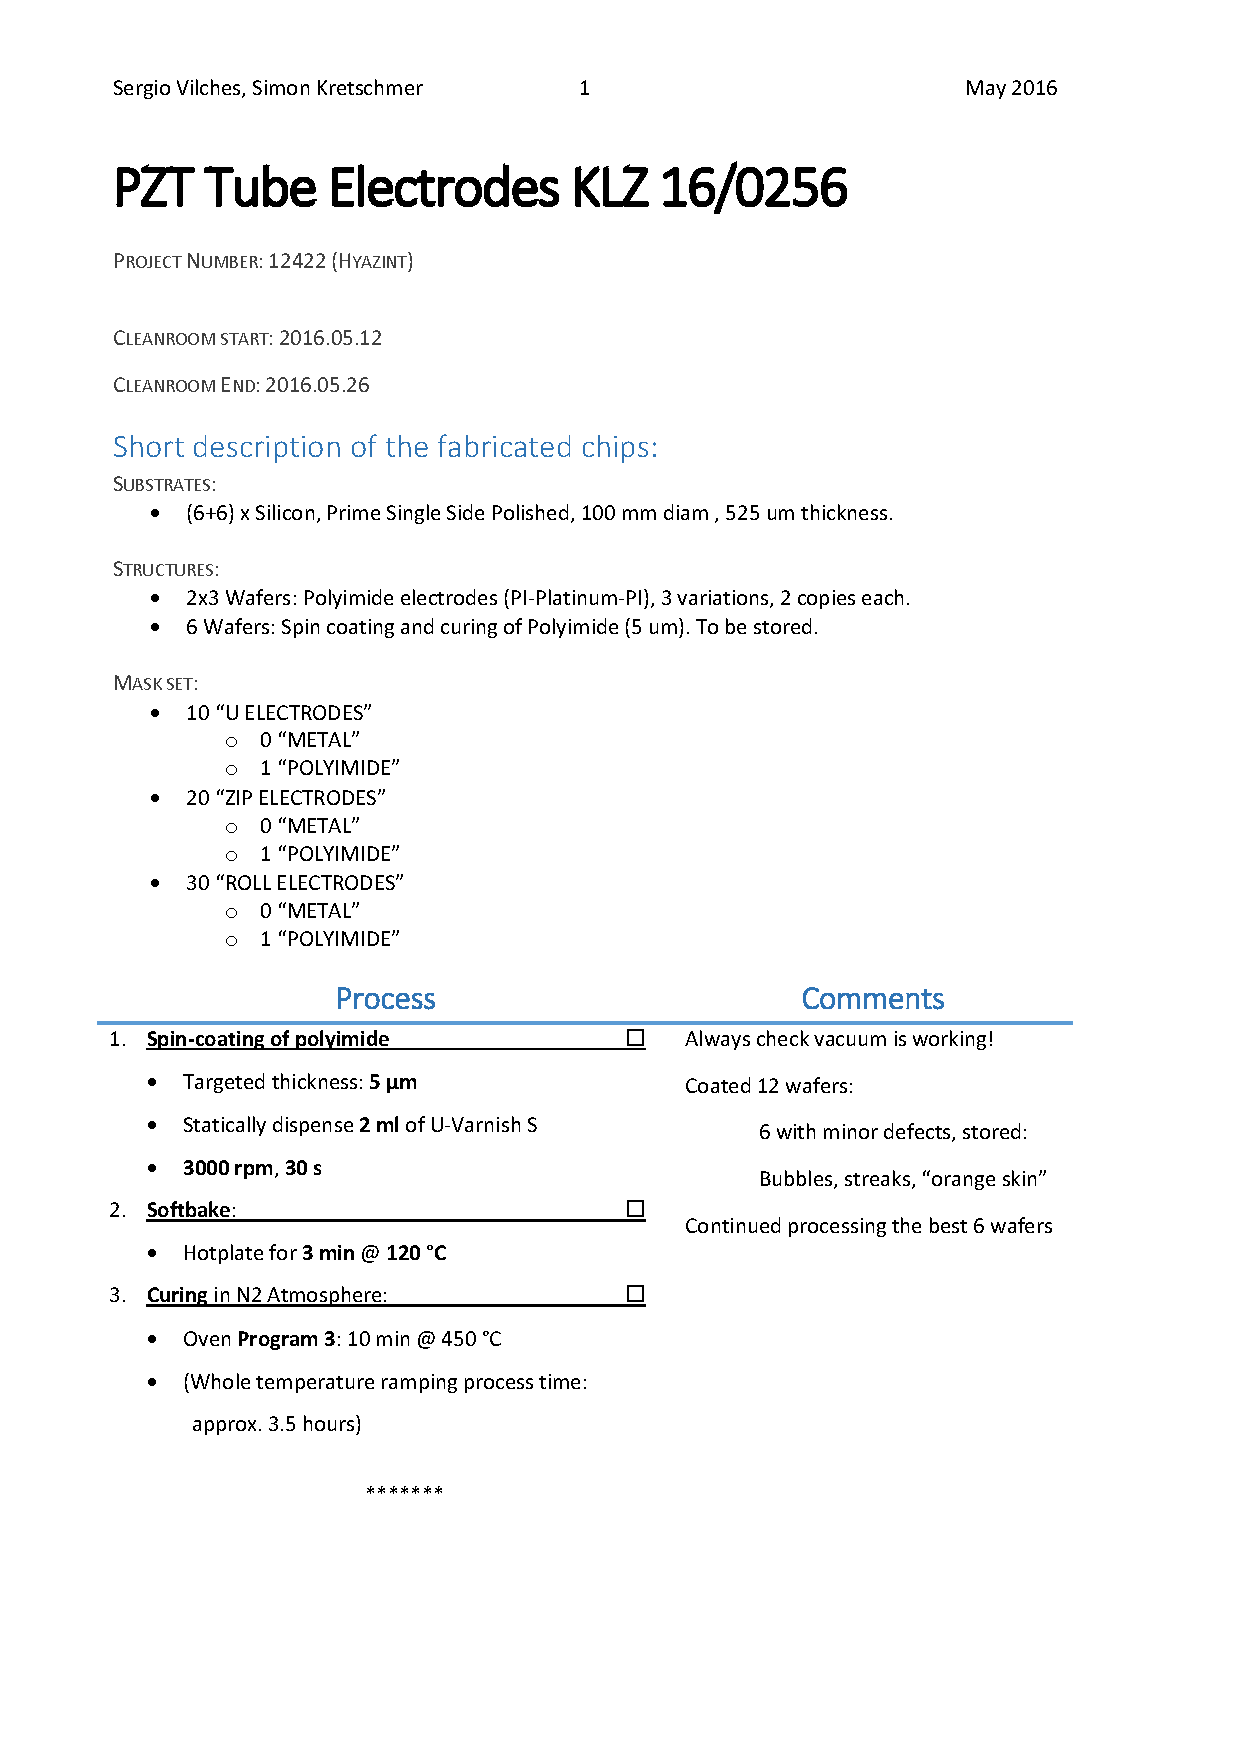
\includepdf[pages={-}]{appendix/runsheetPI.pdf}

\clearpage
\section{Cleanroom processes of the Fiber-GRIN alignment tool}
\begin{figure}[h!]\centering 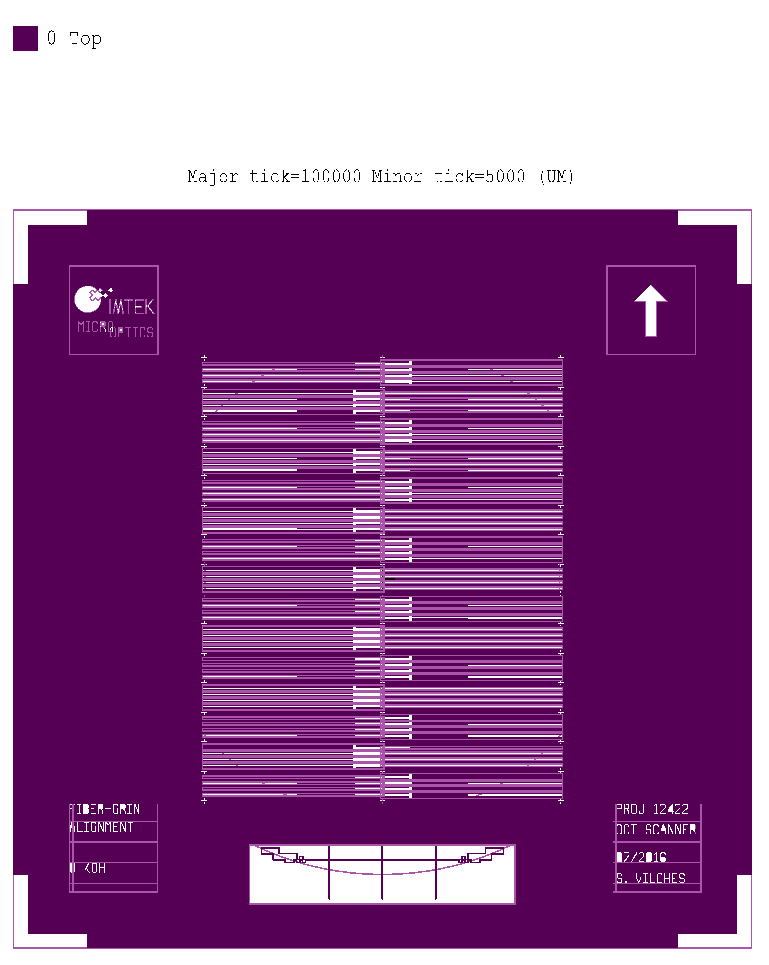
\includegraphics[width=12cm]{appendix/KOH.pdf}
      \caption{Maskset used in the manufacturing of the silicon Fiber-GRIN alignment tool.}
\end{figure}
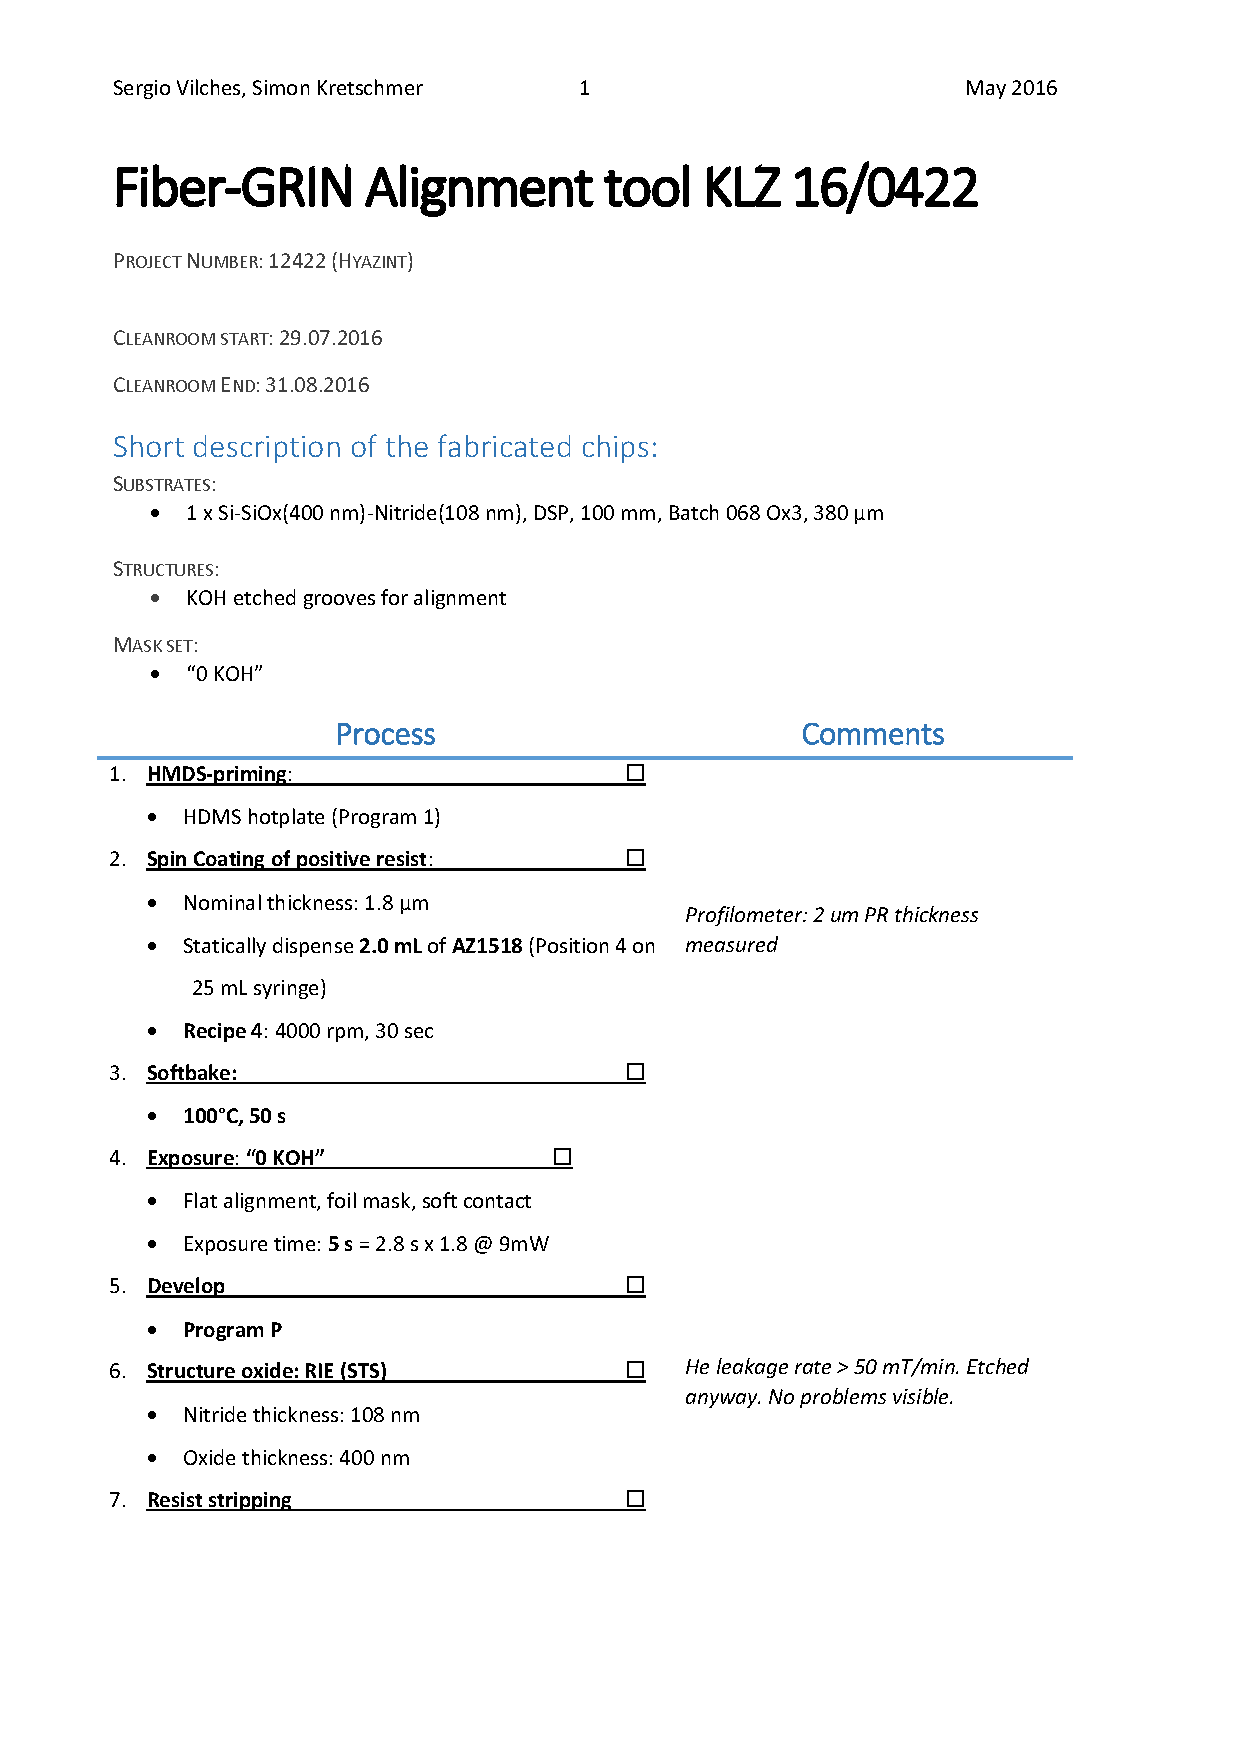
\includepdf[pages={-}]{appendix/runsheetKOH.pdf}

\clearpage
\section{Measurement Setup}
\begin{figure}[h!]\centering 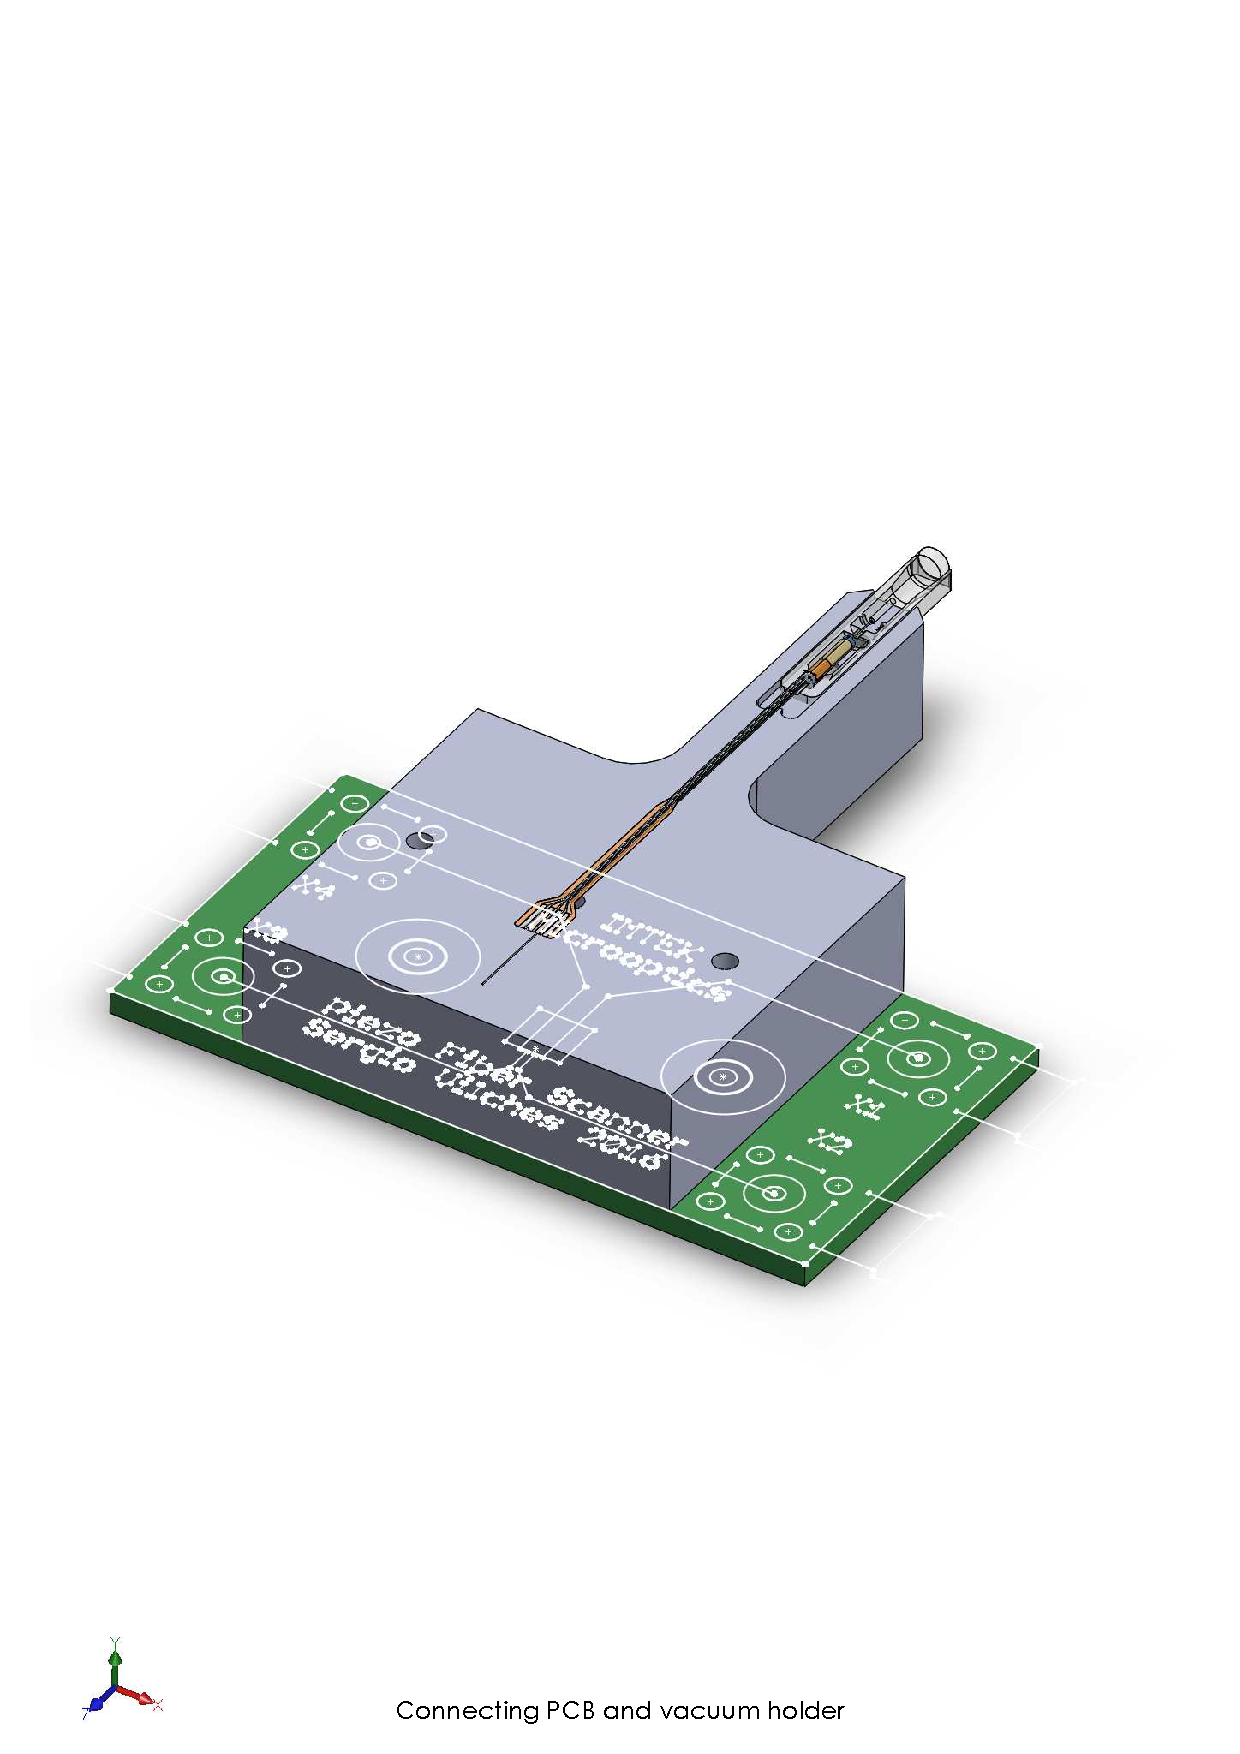
\includegraphics[width=12cm]{appendix/holder.pdf}
      \caption{Render of the breakout PCB and the PMMA vacuum holder with a probe attached.}
\end{figure}
\begin{figure}[h!]\centering 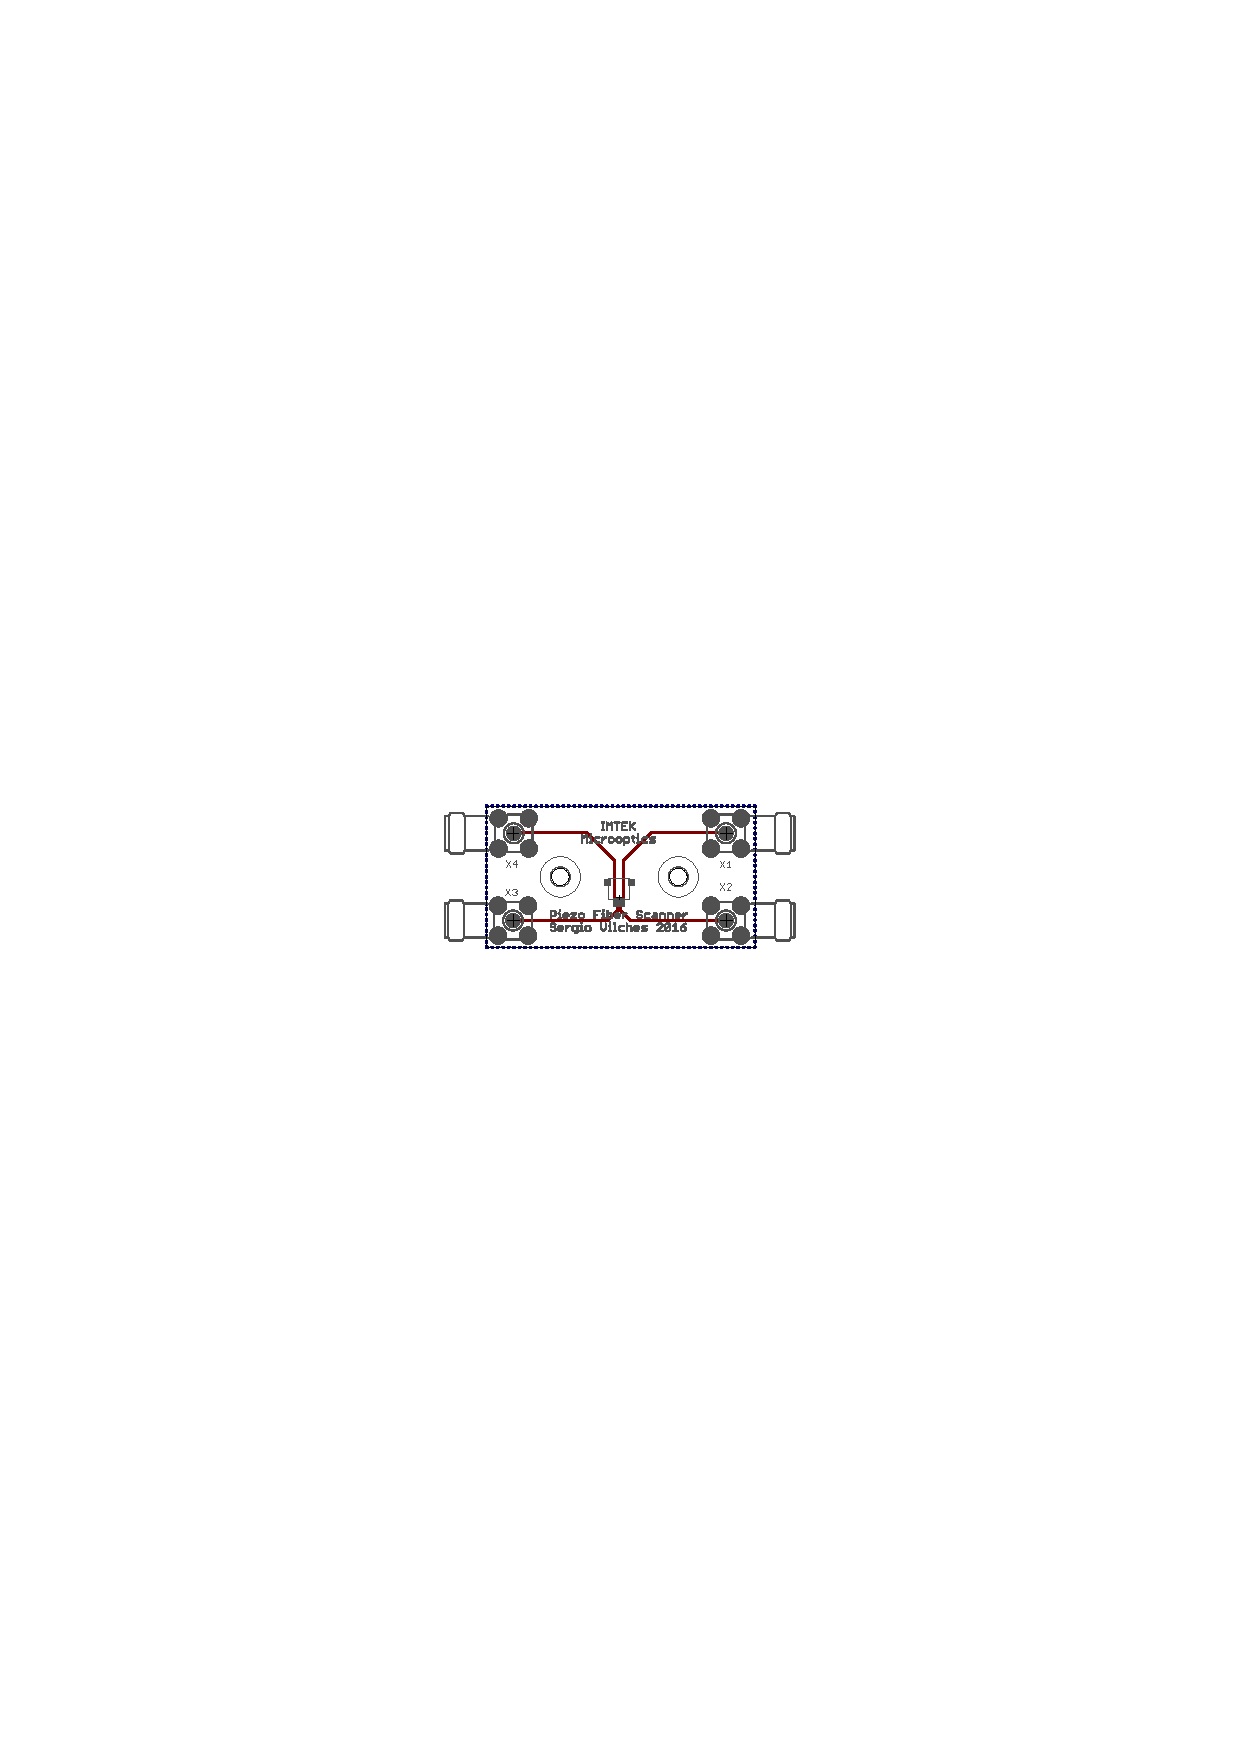
\includegraphics[width=16cm]{appendix/pcb.pdf}
      \caption{Top view of the breakout PCB.}
\end{figure}
\begin{figure}[h!]\centering 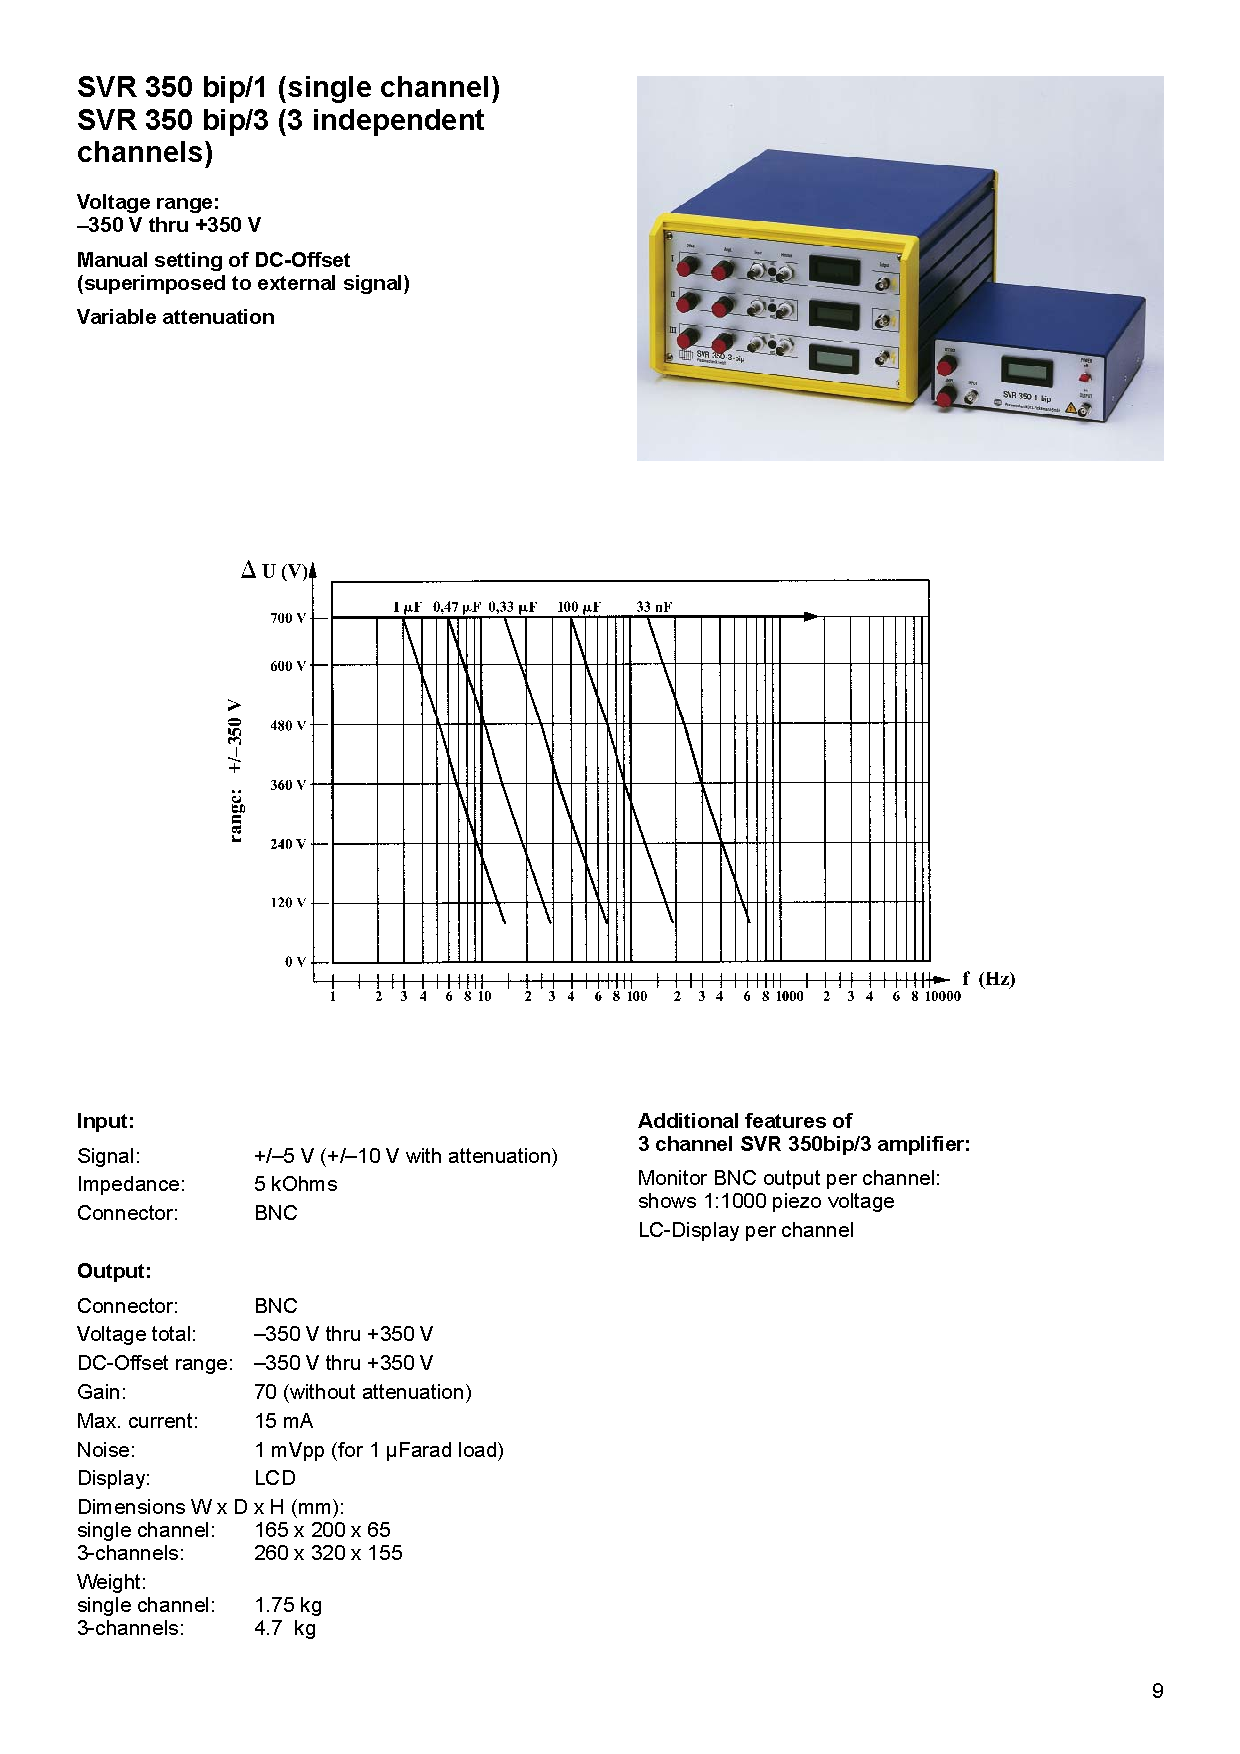
\includegraphics[width=16cm]{appendix/driver.pdf}
      \caption{Datasheet of the high voltage amplifier used to drive the fiber scanner.}
\end{figure}
\begin{figure}[h!]\centering 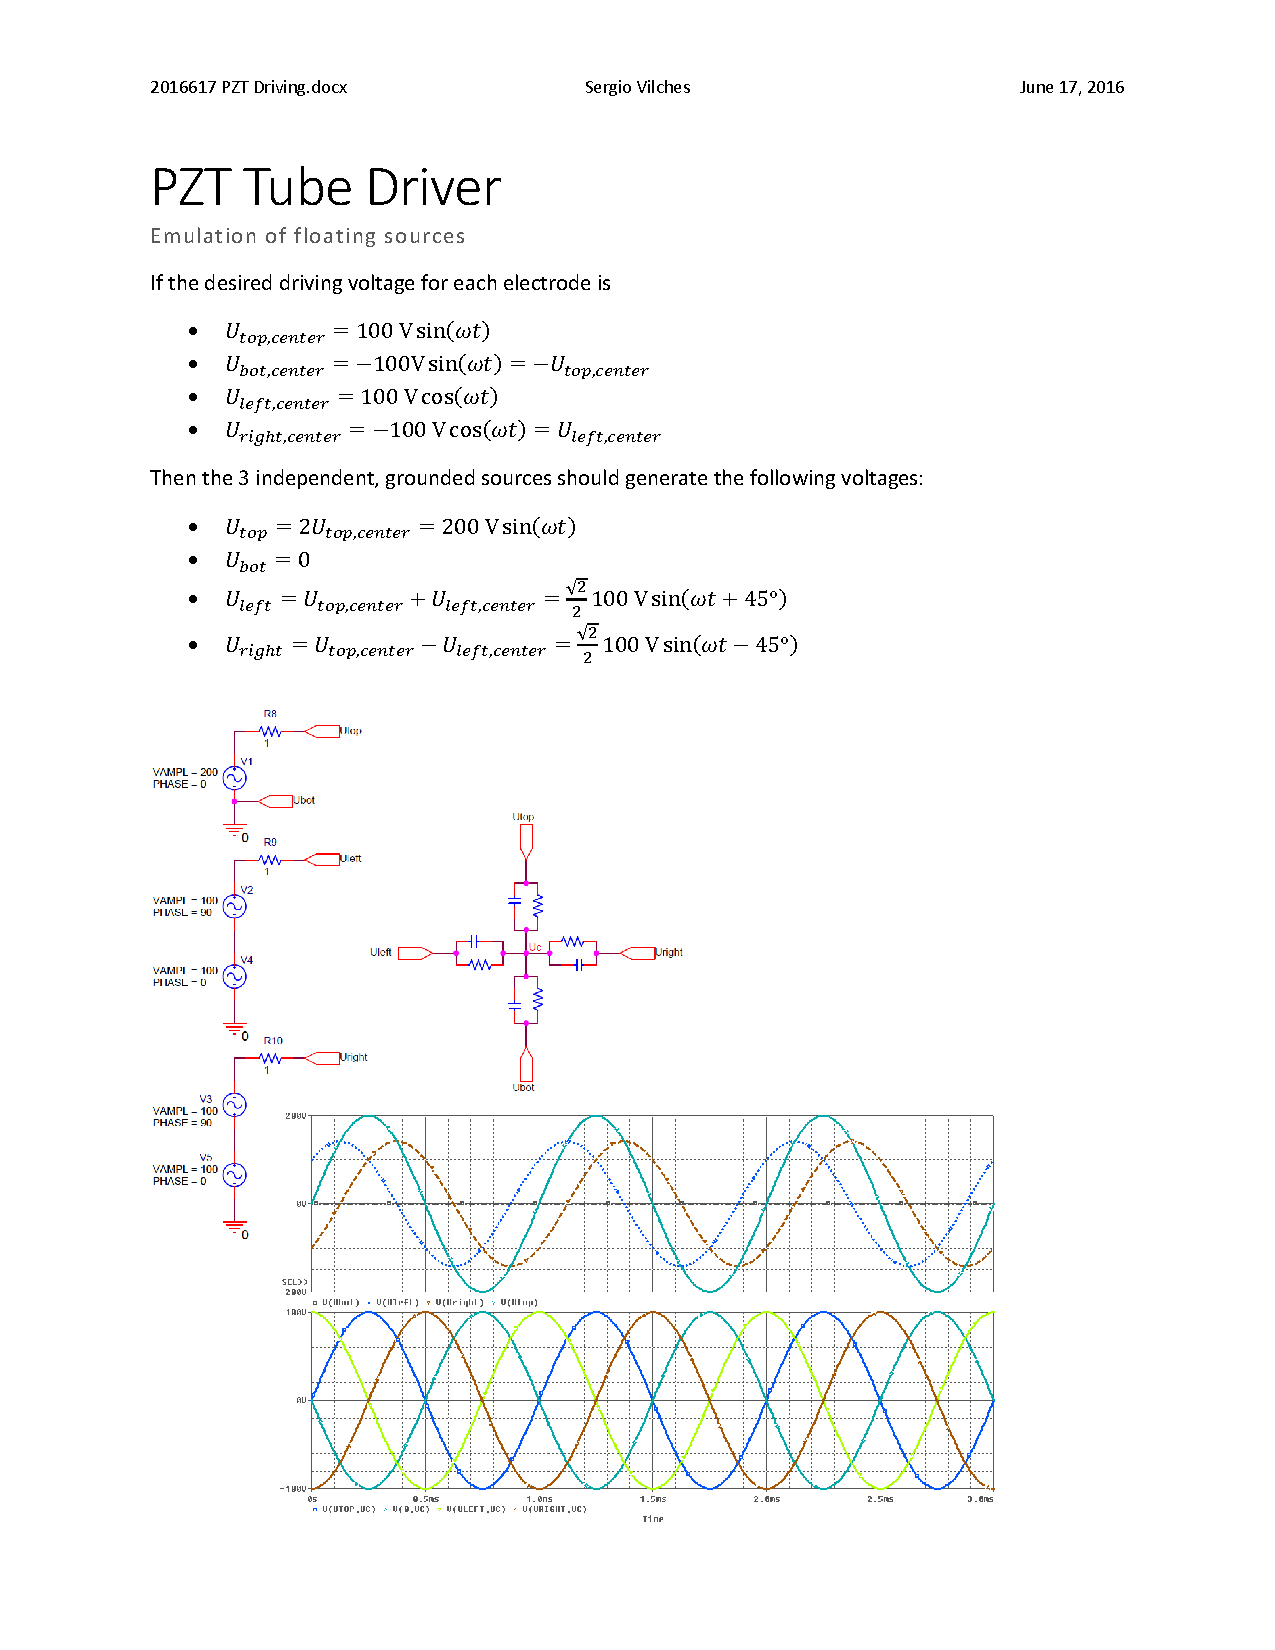
\includegraphics[width=16cm]{appendix/driving.pdf}
      \caption{The fiber scanner needs two independent floating voltage sources to control its position. This documents describes how to emulate two independent floating voltage sources with an amplifier with three common ground outputs using signal processing.}
\end{figure}
\begin{figure}[h!]\centering 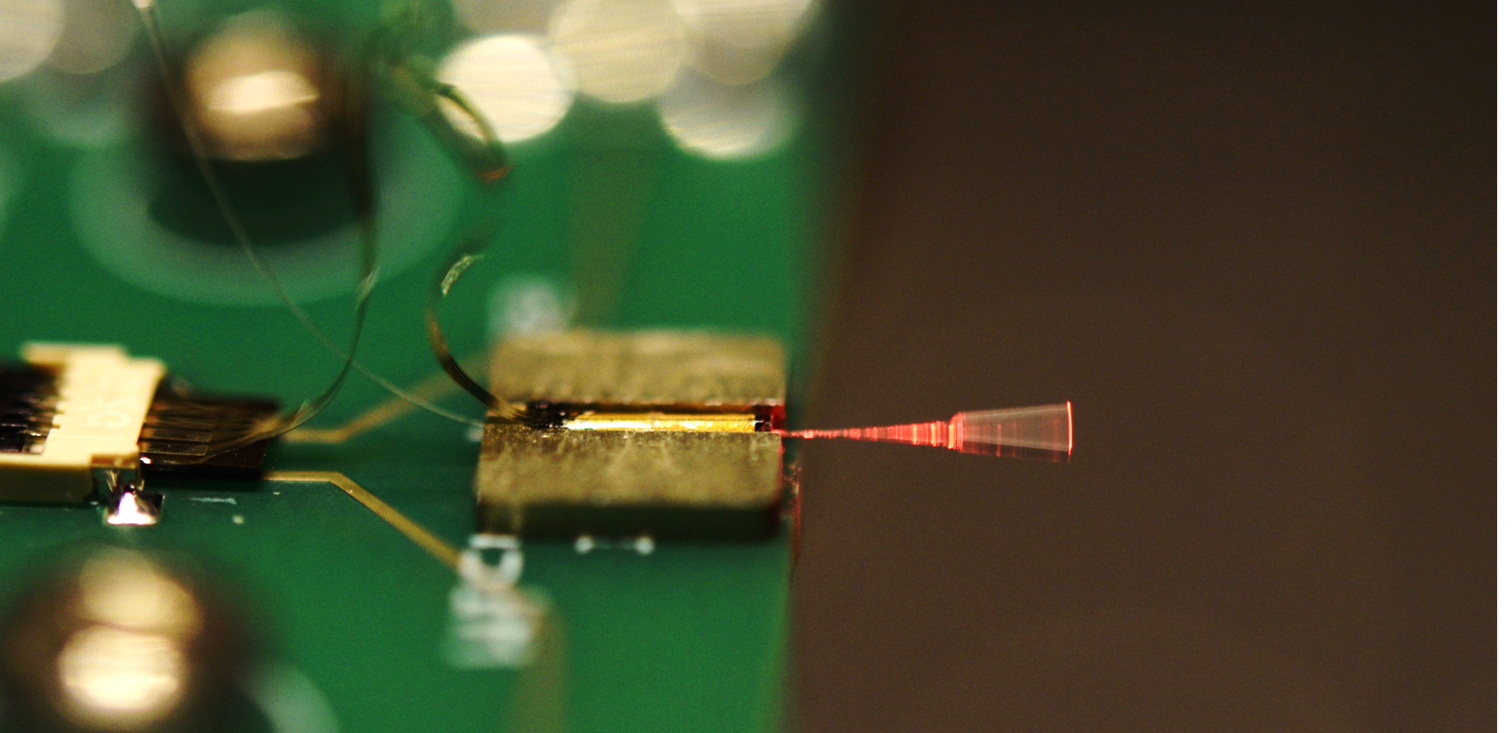
\includegraphics[width=15cm]{appendix/vibrating.png}
      \caption{Fiber scanner mounted in a testbench with a pilot laser coupled into the fiber. By applying a driving voltage with a frequency close to the \textit{Eigenfrequency}, the cantilever enters resonance.}
\end{figure}

\clearpage
\section{Assembly}
\begin{figure}[h!]\centering 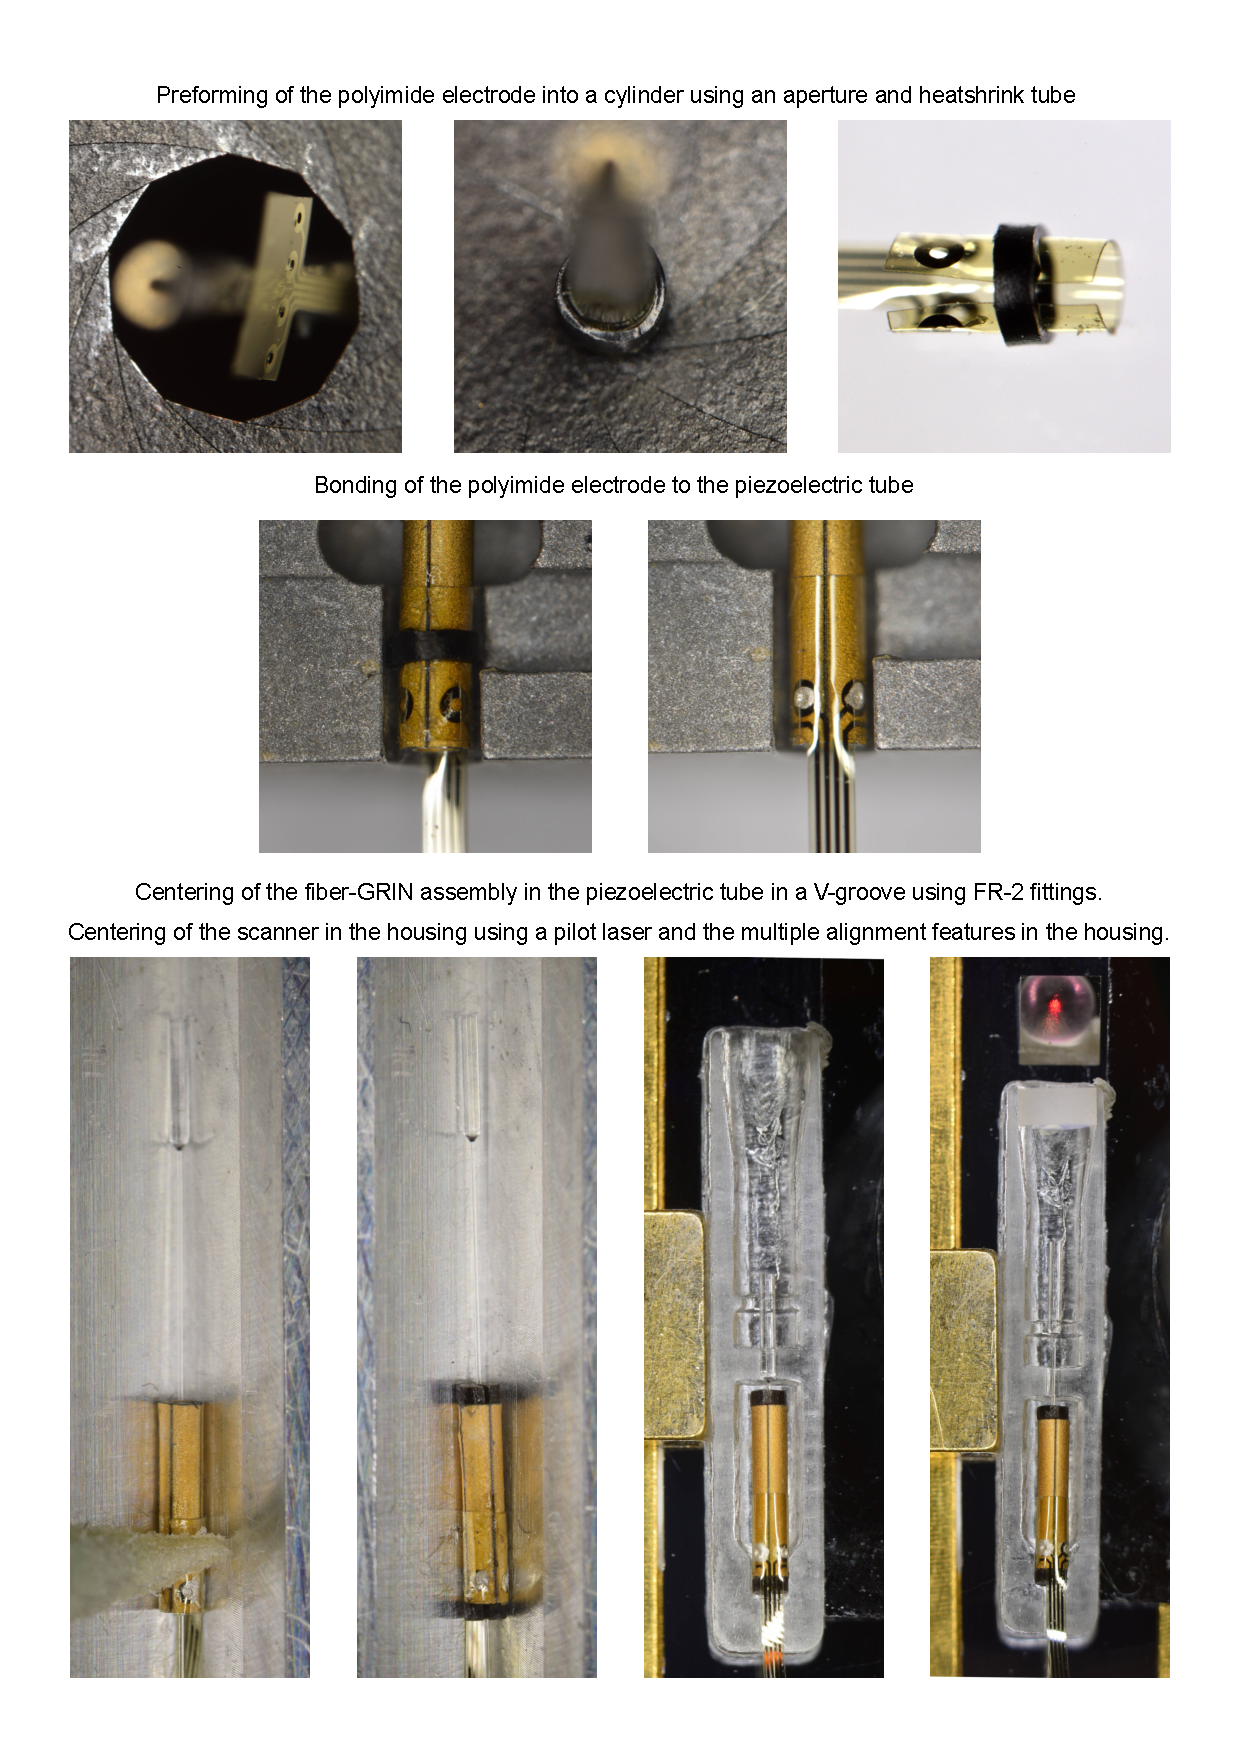
\includegraphics[width=12cm]{appendix/assyPhotos.pdf}
      \caption{Some of the practicalities involved in the assembly of the demonstrator probe.}
\end{figure}

\clearpage
\section{Simulation of a higher NA probe}
\begin{figure}[h!]\centering 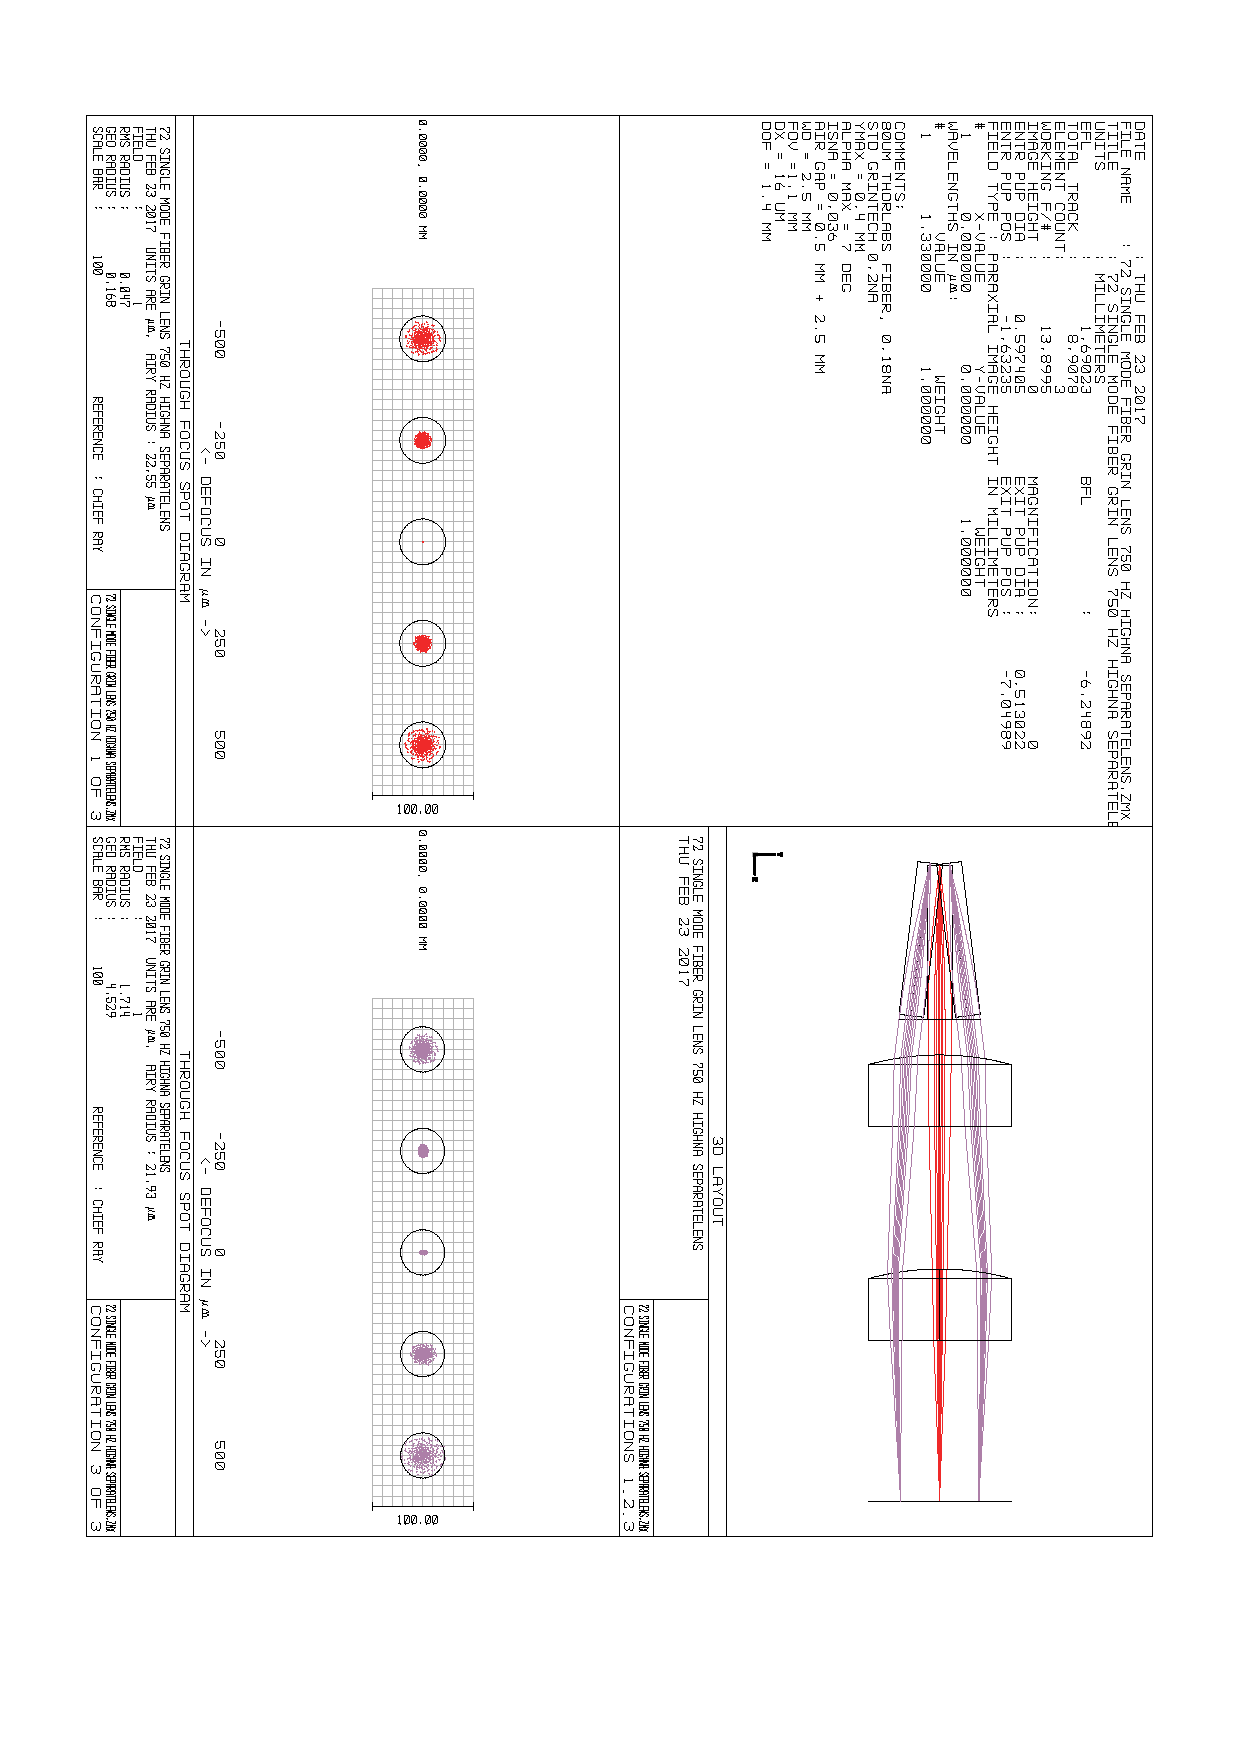
\includegraphics[height=17cm,angle=90,origin=c]{appendix/ZEMAXhigh.pdf}
      \caption{ZEMAX simulation of a probe with higher NA (ISNA = 0.036) by using two objective lenses.}
\end{figure}
\begin{figure}[h!]\centering 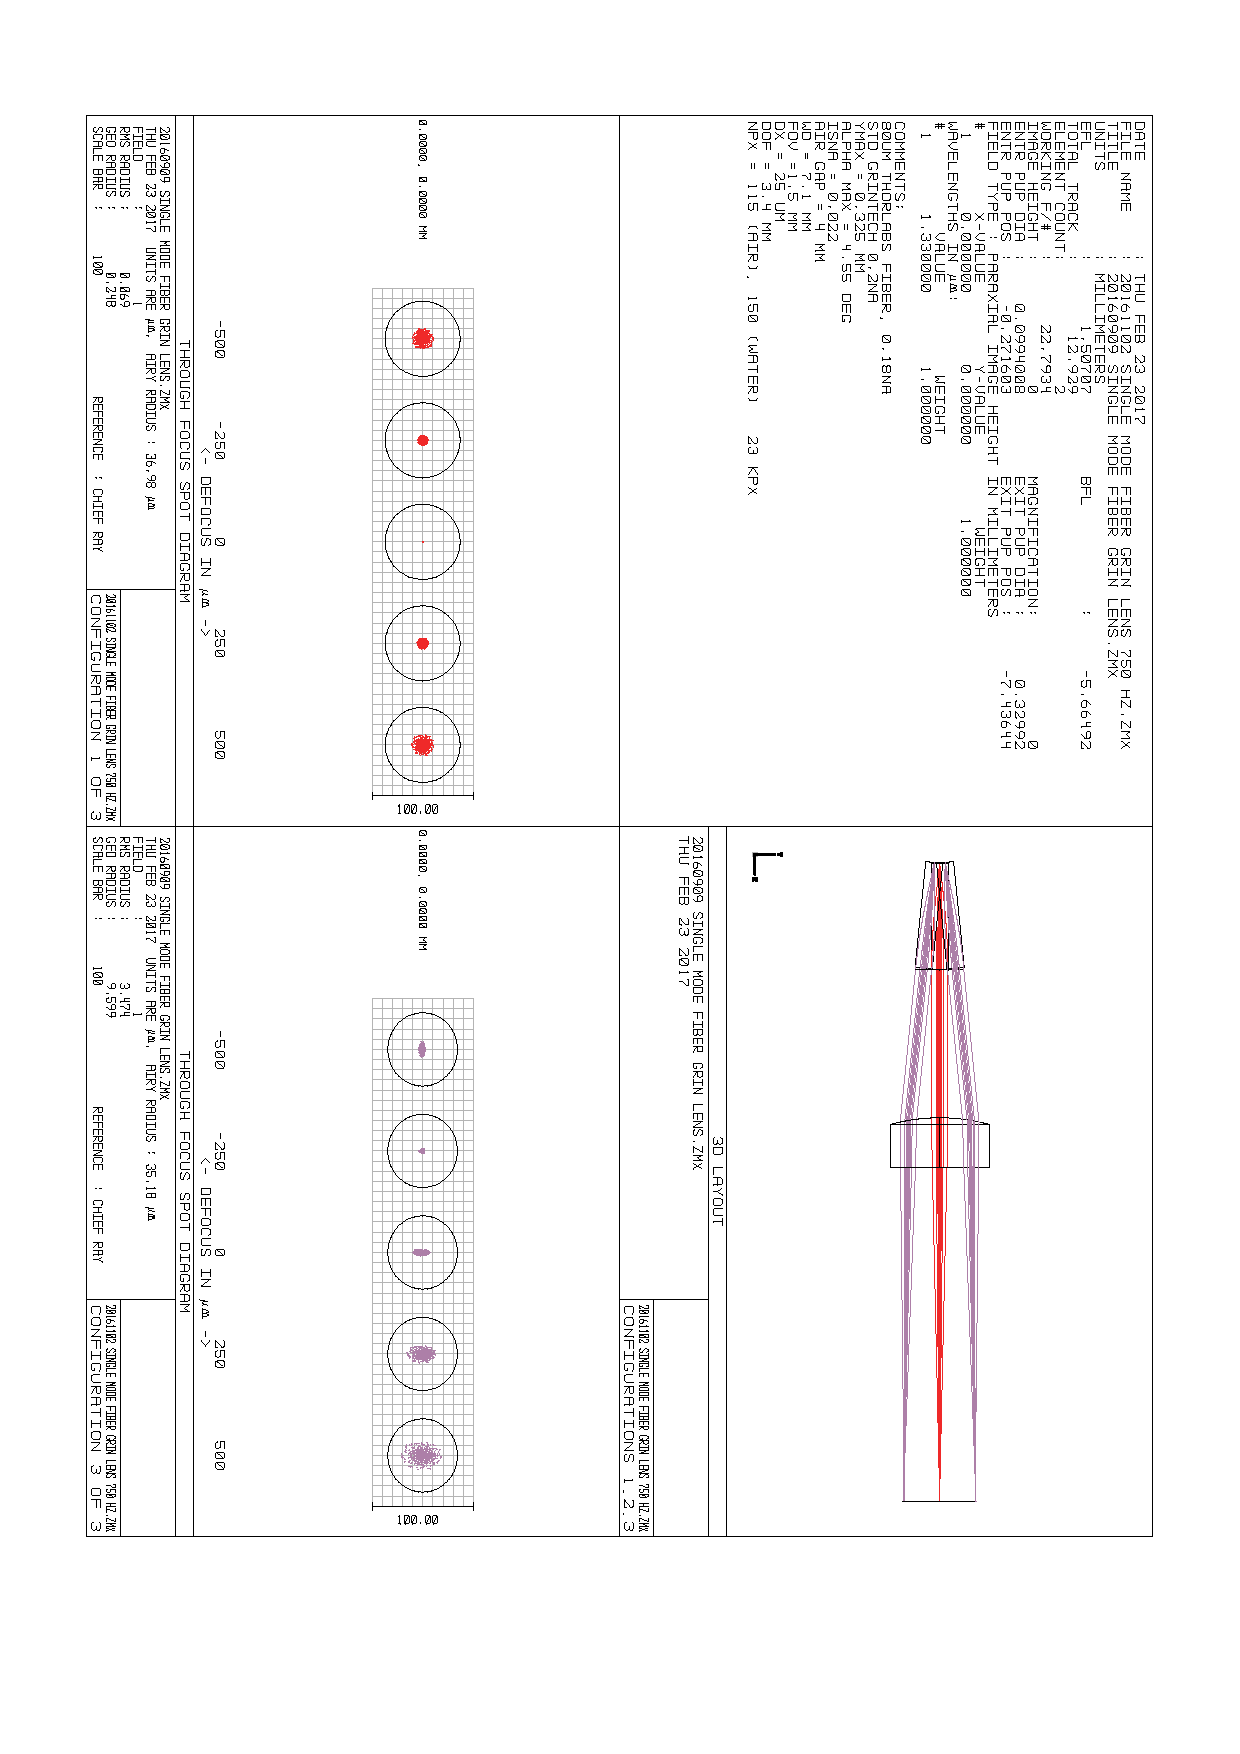
\includegraphics[height=17cm,angle=90,origin=c]{appendix/ZEMAXlow.pdf}
      \caption{ZEMAX simulation of the probe described in this work (ISNA = 0.022), shown for comparison with the previous figure.}
\end{figure}

%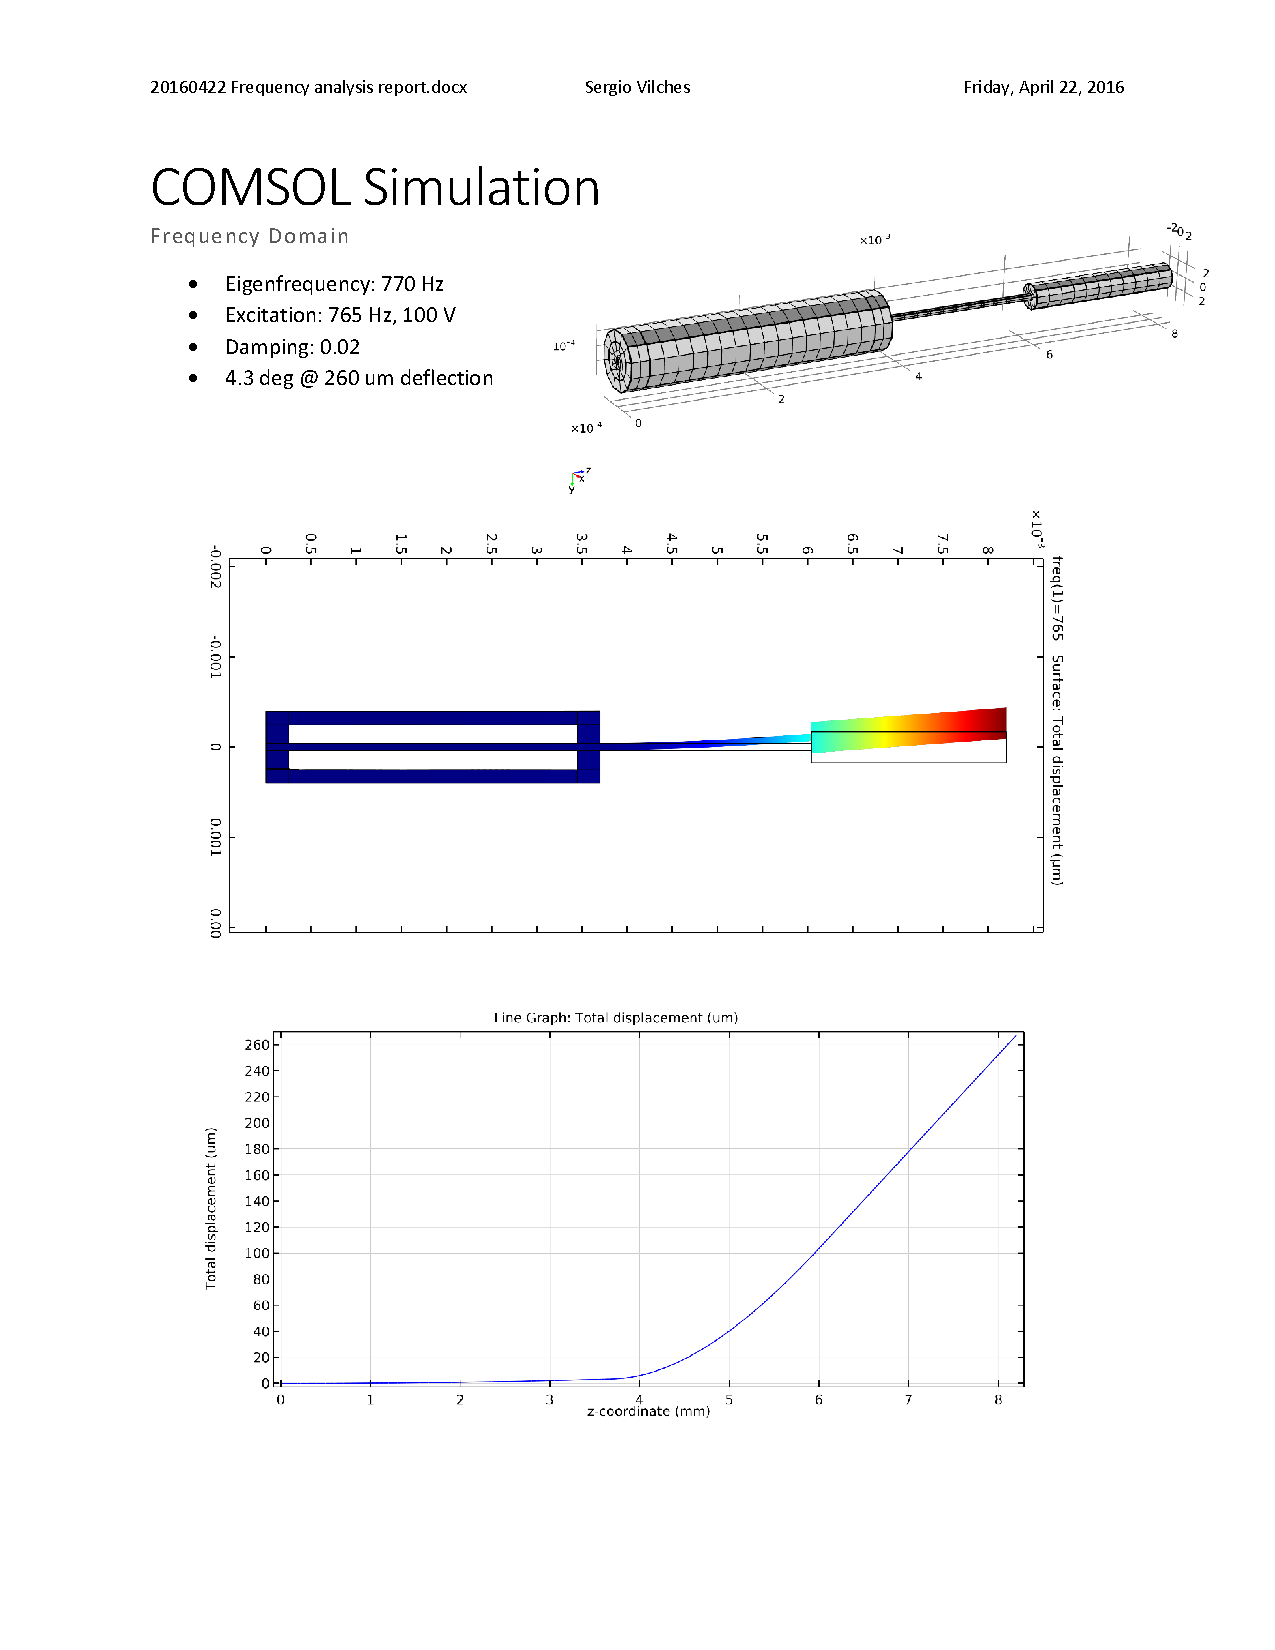
\includepdf{appendix/comsol.pdf}
%
